\documentclass[11pt]{report}
\usepackage{titlesec}
\titleformat{\chapter}
  {\normalfont\LARGE\bfseries}{\thechapter}{1em}{}
\titlespacing*{\chapter}{0pt}{3.5ex plus 1ex minus .2ex}{2.3ex plus .2ex}

\usepackage[margin=1.2in]{geometry}
\usepackage[toc,page]{appendix}
\usepackage{graphicx}
\usepackage{lipsum}
\usepackage{caption}
\usepackage[utf8]{inputenc}
\usepackage[italian]{babel}
\usepackage{verbatim}
\usepackage{colorprofiles}
\usepackage{listings}   %<- per inserire il codice
\usepackage{float}
\usepackage{subcaption}
\usepackage{amsmath}
\usepackage{amsfonts}
\usepackage{listings}
\usepackage{xcolor}
\usepackage{booktabs}
\usepackage{array}

%%%%%%%%%%%%%%%%%%%%%%%%%%%%%%%%%%%%%%%%%%%%%%%%%%%%%%%%%%%%%%%%%%%%
\definecolor{custom_green}{rgb}{0,0.6,0}
\definecolor{codegray}{rgb}{0.5,0.5,0.5}
\definecolor{codepurple}{rgb}{0.58,0,0.82}
\definecolor{backcolour}{rgb}{0.95,0.95,0.92}
\definecolor{custom_blue}{rgb}{  0.05, 0.05, 0.97}
\definecolor{custom_brown}{rgb}{ 0.69, 0.38, 0.10}
\definecolor{custom_purple}{rgb}{0.58, 0.00, 0.82}
\definecolor{custom_orange}{rgb}{0.94, 0.59, 0.09}

\lstdefinestyle{MATLABstyle}{   
    commentstyle=\color{custom_green},
    keywordstyle=\color{magenta},
    numberstyle=\tiny\color{codegray},
    stringstyle=\color{codepurple},
    basicstyle=\ttfamily\footnotesize,
    breakatwhitespace=false,         
    breaklines=true,                 
    captionpos=b,                    
    keepspaces=true,                 
    numbers=left,                    
    numbersep=5pt,                  
    showspaces=false,                
    showstringspaces=false,
    showtabs=false,                  
    tabsize=2
}
\lstdefinelanguage{Cpp}{
      language=C++,
      backgroundcolor=\color{white},  
      basicstyle=\footnotesize \ttfamily \color{black} \bfseries,   
      breakatwhitespace=false,       
      breaklines=true,               
      captionpos=b,                   
      commentstyle=\color{custom_green},   
      deletekeywords={...},          
      escapeinside={\%*}{*)},
      keywordstyle=\color{custom_purple},
      identifierstyle=\color{blue},
      stringstyle=\color{blue},      
      numbers=left,                 
      numbersep=5pt,                  
      numberstyle=\tiny\color{black}, 
      rulecolor=\color{black},        
      showspaces=false,               
      showstringspaces=false,        
      showtabs=false,                
      stepnumber=1,                   
      tabsize=5,                     
      title=\lstname,                 
    }

\lstdefinelanguage{Python}{
    keywords={from, import, def, return, as, in, len, if, elif, else, for, while},
    breakatwhitespace=false,       
    breaklines=true,   
    morecomment=[l]{\#},
    morestring=[b]",
    commentstyle=\color{red},
    keywordstyle=\color{custom_purple},
    numberstyle=\tiny\color{black},
    stringstyle=\color{custom_green},
    basicstyle=\ttfamily\footnotesize,
    captionpos=b,
    showstringspaces=false,        
    showtabs=false,                
    numbers=left,                 
    numbersep=5pt,                  
    numberstyle=\tiny\color{black}, 
    rulecolor=\color{black},                      
    tabsize=5,                     
    title=\lstname,    
}

\lstdefinelanguage{MATLABc}{
    language=MATLAB,
    backgroundcolor=\color{white},  
    basicstyle=\footnotesize \ttfamily \color{black} \bfseries,   
    breakatwhitespace=false,       
    breaklines=true,               
    captionpos=b,
    morestring=[b]",
    commentstyle=\color{custom_green},   
    keywordstyle=\color{custom_blue},
    morekeywords={clearvars},
    deletekeywords={fprintf},
    identifierstyle=\color{black},
    stringstyle=\color{custom_purple},      
    numbers=left,                 
    numbersep=5pt,                  
    numberstyle=\tiny\color{black}, 
    rulecolor=\color{black},        
    showspaces=false,               
    showstringspaces=false,        
    showtabs=false,                
    stepnumber=1,                   
    tabsize=5,                     
    title=\lstname,                 
}
%%%%%%%%%%%%%%%%%%%%%%%%%%%%%%%%%%%%%%%%%%%%%%%%%%%%%%%%%%%%%%%%%%%%




\begin{document}
\captionsetup[figure]{margin=1.5cm,font=small,labelfont={bf},name={Figure},labelsep=colon,textfont={it}}
\captionsetup[table]{margin=1.5cm,font=small,labelfont={bf},name={Table},labelsep=colon,textfont={it}}


\begin{titlepage}
\begin{center}
    {\large \scshape Università Politecnica delle Marche}\\[0.1cm]
    {\large \scshape Ingegneria Informatica e dell'Automazione}\\[0.8cm] 
    \vspace*{0.4cm} 
    {\huge \bfseries Controllo di trazione e sterzata di un veicolo in scala 1:10 mediante radiocomando \par}
    \vspace*{0.8cm}

    
\includegraphics[width=4.5cm]{images/logoUnivpm}\\[0.8cm]

    {\large Corso di}\\[0.1cm]
    {\large \scshape Laboratorio di Automazione}\\[0.1cm]
    Anno accademico 2025-2026\\[0.8cm] 

    \begin{minipage}[t]{0.45\textwidth}
        \begin{flushleft}
            \Large \textbf{Studenti:}\\
            Tarek Naja\\
            Marco Sambughi\\
            Sara Vaccaro
        \end{flushleft}
    \end{minipage}
    \hfill
    \begin{minipage}[t]{0.45\textwidth}
        \begin{flushright}
            \Large \textbf{Professore:}\\
            Andrea Bonci\\[0.6cm]
            \textbf{Dottorando:}\\
            Alessandro Di Biase
        \end{flushright}
    \end{minipage}

    \vfill 

    
\includegraphics[width=2cm]{images/dii_new.png}\\[0.2cm]
    \small Dipartimento di Ingegneria dell'Informazione

\end{center}
\end{titlepage}
\pagenumbering{arabic}
\tableofcontents
\addcontentsline{toc}{chapter}{Introduzione}
\newpage

\pagestyle{plain}

\section*{Introduzione}
Il presente elaborato documenta le fasi di progettazione, sviluppo e validazione del firmware di controllo per un veicolo elettrico in scala 1:10. Nello specifico, il lavoro operativo è stato suddiviso in tre task fondamentali: l'interfacciamento e la decodifica dei segnali radio, la regolazione della trazione per la gestione della velocità e il controllo direzionale dello sterzo, questi ultimi implementati mediante algoritmi di controllo PID.
Nel primo capitolo, viene fornita una descrizione generale del sistema, definendo il contesto operativo e le logiche alla base del controllo della trazione e dello sterzo. Successivamente, il secondo e il terzo capitolo offrono una panoramica dettagliata dell'architettura hardware e degli ambienti software impiegati, delineando tutti i requisiti strumentali necessari per la riproduzione del setup sperimentale. 
Al suo interno viene dapprima analizzata la struttura generale del codice, per poi scendere nel dettaglio degli algoritmi sviluppati per l'acquisizione e l'elaborazione dei segnali del radiocomando, 
illustrando l'impostazione dei timer, il calcolo del Duty Cycle e la gestione degli interrupt. A partire da queste fondamenta, vengono discussi i codici e le librerie specifiche implementate mediante l'utilizzo di regolatori PID, analizzando dapprima l'erogazione della trazione tramite la lettura dell'encoder, e successivamente il controllo direzionale dello sterzo, inclusa la sua necessaria calibrazione meccanica. 
Per dimostrare la validità del lavoro svolto, ciascuna di queste tre macro-fasi di implementazione software, è corredata da un'analisi dedicata ai test sul campo e ai risultati ottenuti, 
permettendo di verificare concretamente la prontezza e la stabilità della risposta dinamica del veicolo. Infine, la relazione si conclude con una panoramica sui possibili sviluppi futuri, delineando potenziali miglioramenti e ottimizzazioni per le successive evoluzioni del prototipo.

\newpage
\chapter{Descrizione del sistema}
La seguente relazione si basa sull'analisi dell'architettura di comunicazione via radio tra radiocomando e microcontrollore. Nel dettaglio, il trasmettitore impiega onde elettromagnetiche per l'invio dei pacchetti dati, sfruttando la modulazione di un'onda portante che codifica le informazioni variando parametri dell'onda stessa, quali l'ampiezza, la frequenza o la fase. L'espressione matematica dell'onda portante è definita dalla seguente funzione:

\begin{equation}
    s(t) = A \cos(2\pi f_c t + \phi)
\end{equation}

\noindent dove:
\begin{itemize}
    \item $A$: ampiezza dell'onda;
    \item $f_c$: frequenza portante;
    \item $t$: tempo;
    \item $\phi$: fase iniziale.
\end{itemize}

\noindent
L'azione dell'utente sui comandi del radiocomando genera una sequenza di bit (segnale elettrico), che l'antenna del trasmettitore provvede a convertire in onda elettromagnetica, irradiandola nello spazio a una determinata frequenza $f$. Il modulo ricevitore, essendo sintonizzato sulla stessa frequenza, intercetta il segnale e lo riconverte nel formato elettrico. Questi dati vengono poi inoltrati al microcontrollore, il quale ha il compito di interpretare le istruzioni e comandare l'hardware per eseguire determinate azioni. 
\noindent
Per la traduzione pratica dei comandi, il microcontrollore impiega la modulazione a larghezza di impulso (PWM). Il parametro fondamentale per questa tecnica è il \textit{Duty Cycle}, calcolato come segue:

\begin{equation}
    \text{Duty Cycle (\%)} = \frac{T_{on}}{T_{on} + T_{off}} \times 100
\end{equation}

\noindent dove $T_{on}$ è la durata dell'impulso ``alto'', $T_{off}$ la durata dell'impulso ``basso'' e la loro somma definisce il periodo totale dell'onda.
\noindent
Per quanto riguarda l'analisi della traiettoria del veicolo, si adotta il modello cinematico della bicicletta, approssimando la dinamica del veicolo a quattro ruote riducendola a due. Le equazioni cinematiche descrivono il moto attraverso le variabili di posizione $(x,y)$ e l'angolo di orientamento della vettura. Considerando costante la velocità $v$ del veicolo, l'assenza di slittamento e che l'intera rotazione del veicolo avvenga attorno al CIR (Centro Istantaneo di Rotazione), il modello viene descritto dal seguente sistema:

\begin{equation}
    \begin{cases}
        \dot{x}(t) = v \cos(\theta) \\
        \dot{y}(t) = v \sin(\theta) \\
        \dot{\theta}(t) = \frac{v}{L} \tan(\delta)
    \end{cases}
\end{equation}

\noindent I parametri fondamentali del modello sono:
\begin{itemize}
    \item $L$: distanza tra asse anteriore e posteriore (passo);
    \item $\delta$: angolo di sterzata (ruote anteriori);
    \item $\theta$: angolo di imbardata del veicolo;
    \item $v$: velocità della macchina;
    \item $\dot{x}, \dot{y}$: velocità nei due assi (derivate della posizione rispetto al tempo).
\end{itemize}
\noindent
Nel caso in cui si considerasse lo slittamento si passerebbe ad un modello dinamico e la velocità di rotazione non dipenderebbe più solo dalla geometria. Il modello descritto quindi è una semplificazione del modello reale, ma risulta uno strumento efficace per comprendere la cinematica di base del veicolo e la traiettoria in funzione dell'angolo di sterzo, sfruttando unicamente due assi.
\section{Controllo veicolo}
Nelle prossime sezioni verranno analizzate, dal punto di vista teorico, le tecniche di controllo
utilizzate per la gestione degli attuatori presenti sul veicolo.

\subsection{Controllo della trazione}
Per il controllo della trazione, ovvero la regolazione della velocità longitudinale del veicolo, si è optato per un sistema di controllo in retroazione (\textit{closed-loop}). Tale architettura risulta fondamentale non solo per garantire il preciso inseguimento della velocità di riferimento, ma anche per compensare i disturbi esterni non prevedibili, quali le variazioni di attrito del terreno, le pendenze o le cadute di tensione della batteria durante l'erogazione di corrente.
\noindent Il sistema misura costantemente la velocità reale del veicolo e la confronta con la velocità di riferimento, generando un segnale di errore $e(t)$ da minimizzare:

\begin{equation}
    e(t) = v_{\text{target}} - v_{\text{reale}}
\end{equation}
\noindent Il feedback di velocità è fornito da un encoder incrementale calettato sull'albero motore: il sensore genera una serie di impulsi che vengono conteggiati dal microcontrollore all'interno di un periodo di campionamento a tempo fisso. Dalla derivata discreta di questi conteggi si ricava l'effettiva velocità di rotazione del rotore.
\noindent Per minimizzare l'errore $e(t)$ e calcolare lo sforzo di controllo da applicare al motore, tradotto poi nel \textit{Duty Cycle} del segnale PWM, viene impiegato un controllore PID (Proporzionale-Integrale-Derivativo). La legge di controllo nel dominio del tempo continuo è descritta dalla seguente equazione:

\begin{equation}
    u(t) = K_p \cdot e(t) + K_i \int e(t) \, dt + K_d \frac{de(t)}{dt}
\end{equation}

\noindent dove $u(t)$ rappresenta l'azione di comando generata dal controllore, mentre $K_p$, $K_i$ e $K_d$ sono rispettivamente le costanti di guadagno dell'azione proporzionale, integrale e derivativa. Nello specifico:

\begin{itemize}
    \item \textbf{Guadagno proporzionale ($K_p$):} fornisce un'uscita di controllo direttamente proporzionale all'errore istantaneo. Aumentare il guadagno $K_p$ rende il sistema più reattivo e riduce il tempo di salita. Tuttavia, da sola non è sufficiente a garantire il perfetto inseguimento del riferimento: un'azione puramente proporzionale lascia un errore a regime e, se eccessiva, induce forti oscillazioni e instabilità.
    
    \item \textbf{Guadagno integrale ($K_i$):} somma l'errore nel tempo, tenendo conto della ``storia'' del sistema. Il suo scopo fondamentale è annullare completamente l'errore a regime. Tuttavia, un accumulo prolungato di questo termine, ad esempio durante la fase di avvio o nel caso in cui le ruote slittino senza far muovere il veicolo, porta a un eccessivo incremento dell'azione di controllo. Questo si traduce in partenze improvvise o risposte sproporzionate non appena il target cambia, problematica che nel software è stata mitigata azzerando il termine integrale in specifiche condizioni di sicurezza.
    
    \item \textbf{Guadagno derivativo ($K_d$):} reagisce alla velocità di variazione dell'errore, anticipandone l'andamento futuro. Funge essenzialmente da ``smorzatore'', con lo scopo di contrastare le eventuali oscillazioni introdotte dalle componenti precedenti. Tuttavia, per il controllo longitudinale di veicoli di questa scala, l'azione derivativa risulta spesso superflua o persino controproducente, in quanto tende ad amplificare matematicamente le normali micro-vibrazioni meccaniche o i piccoli scatti letti dall'encoder. Per questo motivo, è prassi comune nella robotica mobile di base porre direttamente $K_d = 0$, semplificando l'architettura a un più robusto e stabile controllore PI.
\end{itemize}

\begin{figure}[H]
    \centering
    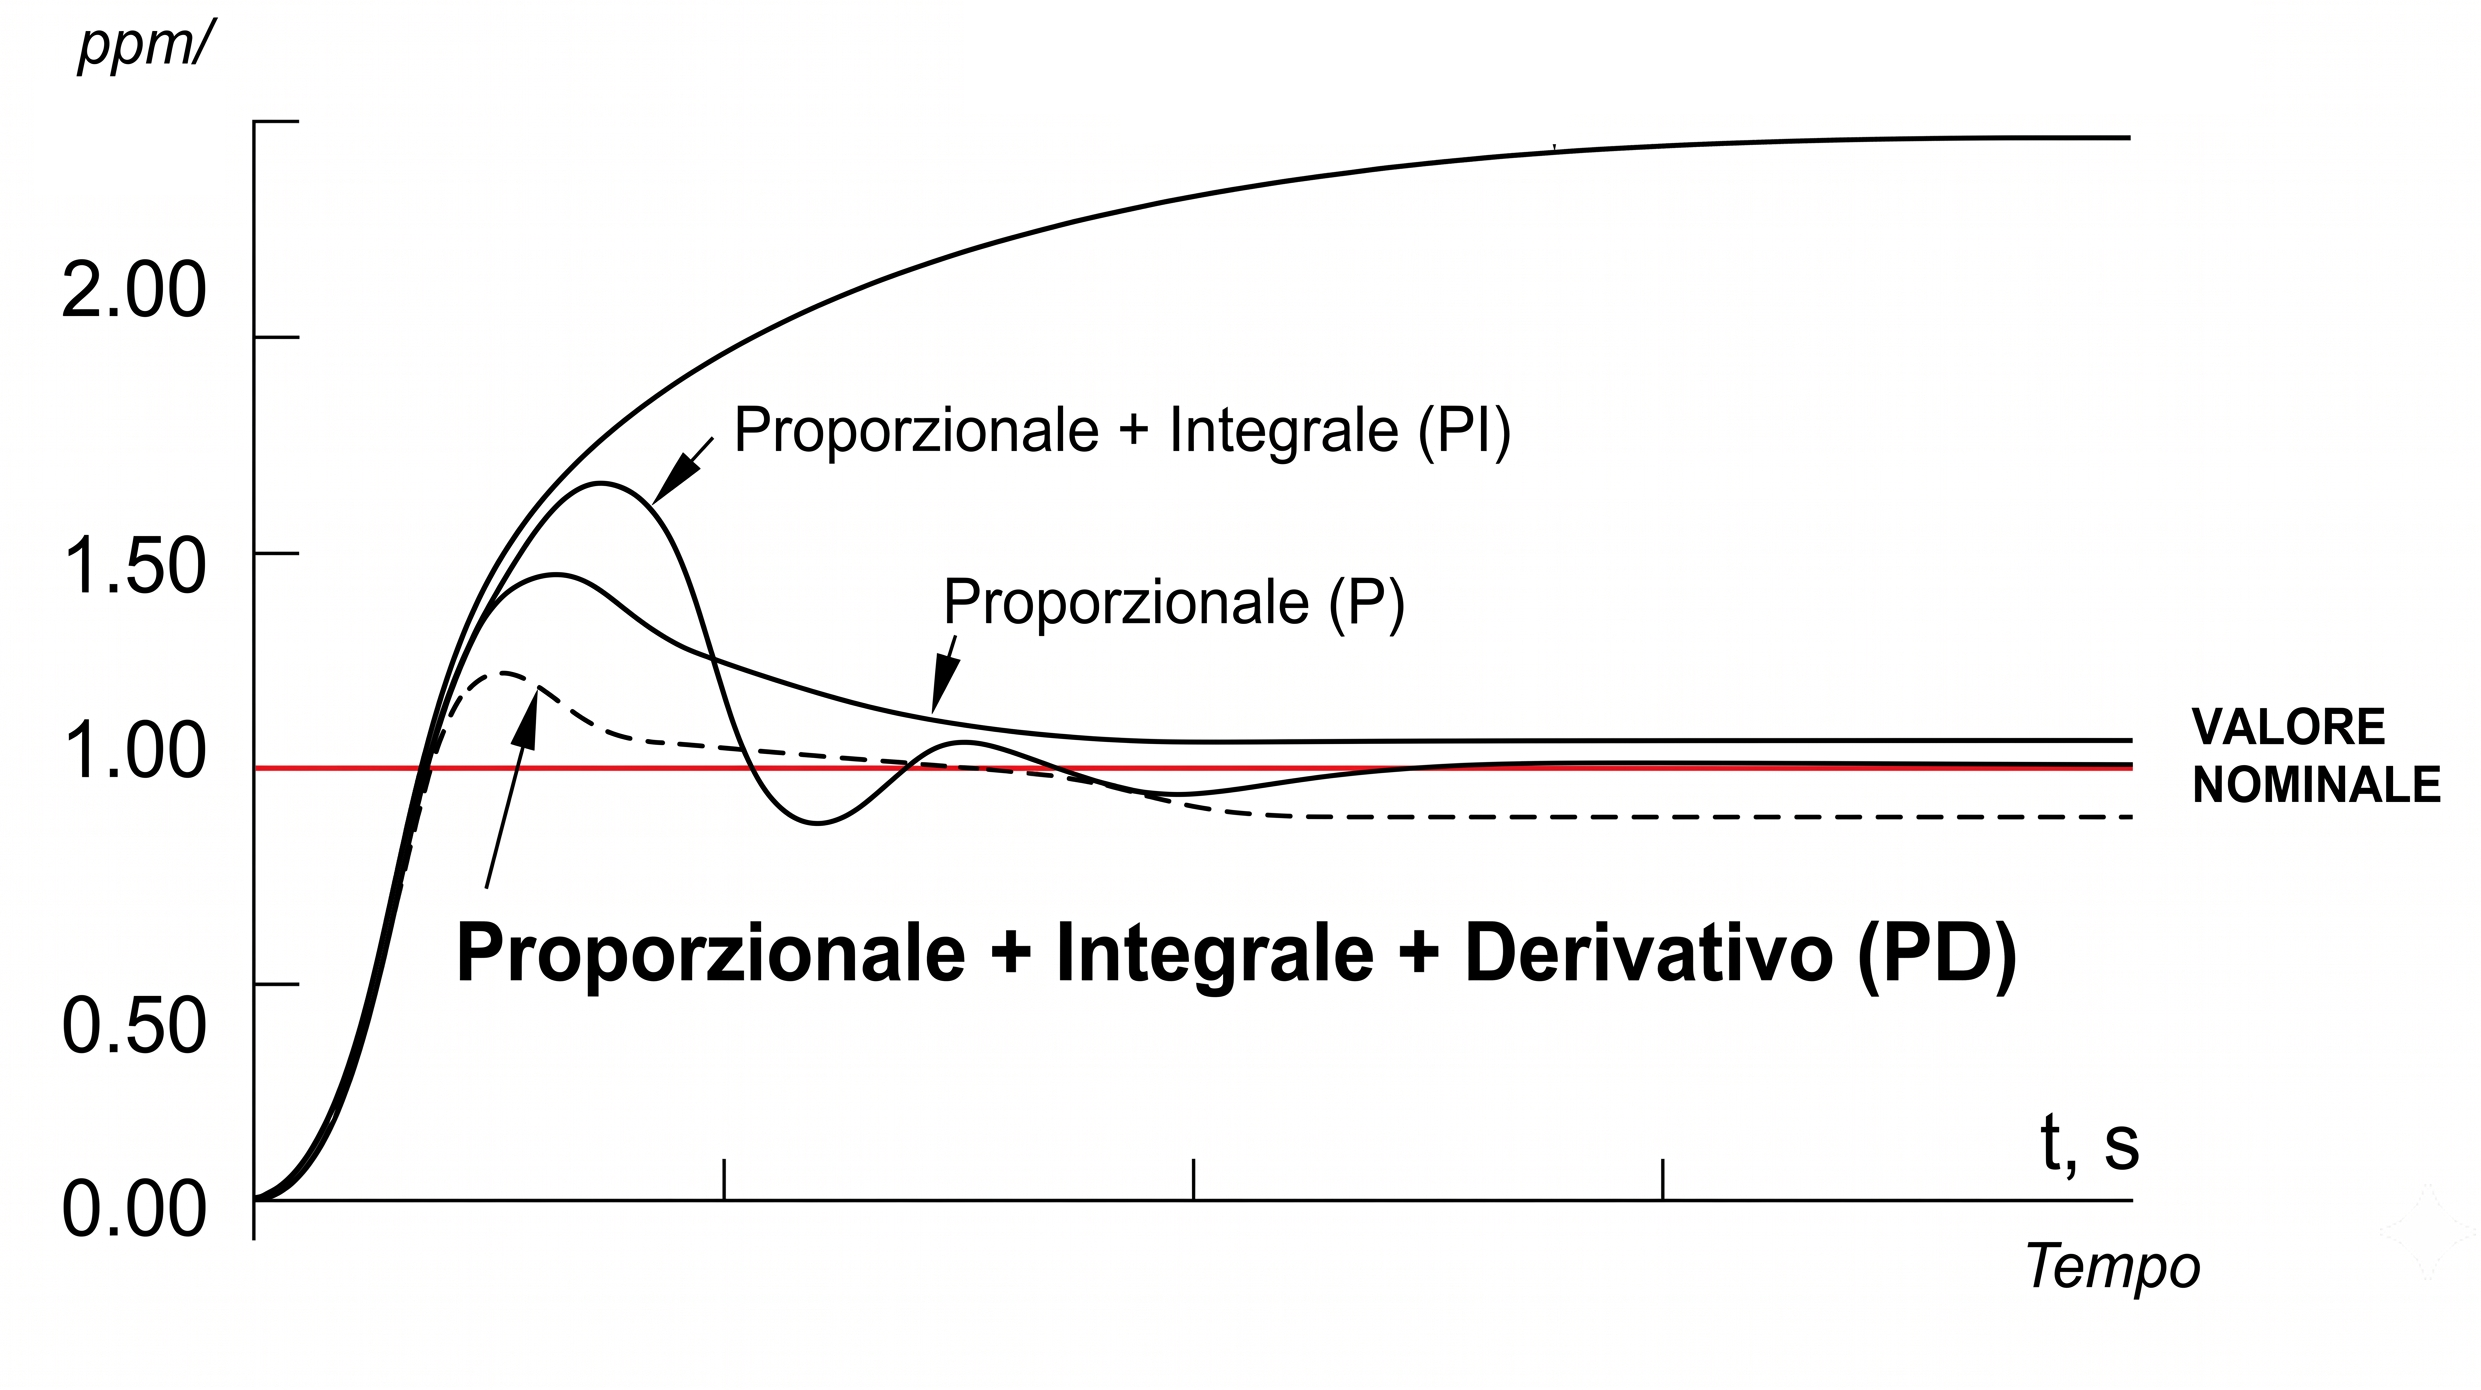
\includegraphics[width=0.7\textwidth]{images/PID} 
    \captionsetup{labelsep=none}
    \caption{}
    \label{fig:telaio}
\end{figure}

\noindent La determinazione dei parametri ottimali ($K_p$, $K_i$, $K_d$) prende il nome di calibrazione o \textit{tuning}.
\noindent Per la dinamica del veicolo in esame, tale procedura è stata condotta mediante calibrazione empirica in laboratorio. Partendo da valori conservativi e analizzando visivamente e tramite telemetria la risposta del motore alle variazioni di velocità richieste dal radiocomando, i guadagni sono stati ottimizzati per garantire l'inseguimento del target senza innescare instabilità.

\begin{figure}[H]
    \centering
    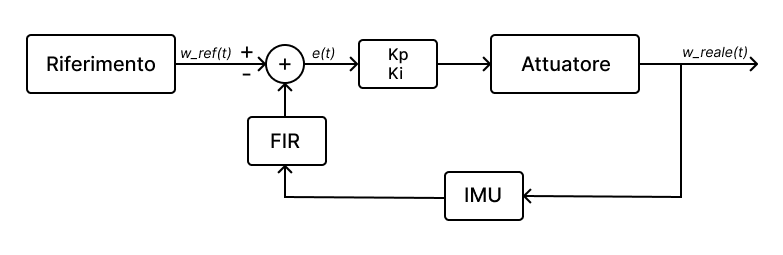
\includegraphics[width=1.0\textwidth]{images/Controllotrazione} 
    \captionsetup{labelsep=none}
    \caption{}
    \label{fig:telaio}
\end{figure}

\subsection{Controllo dello sterzo}
La gestione direzionale del veicolo è affidata al sistema di sterzo delle ruote anteriori e ai segnali inviati dal radiocomando. L'attuazione meccanica è realizzata mediante un servomotore, un tipo particolare di motore che, agendo sui braccetti dello sterzo, è in grado di ruotare in una specifica posizione e mantenerla. Inoltre, in questo prototipo è stato implementato un controllo a ciclo chiuso per garantire la massima precisione nell'inseguimento della traiettoria e compensare i disturbi dinamici come gli attriti del terreno. Di conseguenza, il controllo prevede l'utilizzo di un regolatore PID, implementato all'interno del microcontrollore STM32. 
\noindent Il controllore riceve in ingresso l'errore $e(t)$, definito come la differenza tra l'angolo di sterzo di riferimento richiesto $\delta_{\text{ref}}(t)$, letto dal radiocomando, e l'angolo reale misurato dai sensori di bordo $\delta_{\text{reale}}(t)$:

\begin{equation}
    e(t) = \delta_{\text{ref}}(t) - \delta_{\text{reale}}(t)
\end{equation}

\noindent L'azione correttiva calcolata dall'algoritmo PID viene tradotta in un segnale di pilotaggio PWM inviato al servomotore. Per questa tipologia di attuatori, il controllo della posizione non dipende dal \textit{Duty Cycle} percentuale classico, bensì dalla larghezza assoluta dell'impulso positivo $T_{on}$ all'interno di un periodo fisso di 20 ms, corrispondente ad una frequenza di 50 Hz.


\begin{figure}[H]
    \centering
    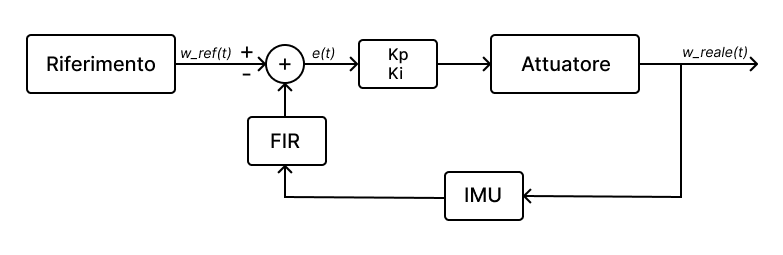
\includegraphics[width=1.0\textwidth]{images/Controllotrazione} 
    \captionsetup{labelsep=none}
    \caption{}
    \label{fig:telaio}
\end{figure}

\newpage
\chapter{Hardware}
\label{Hardware}
Nel presente capitolo viene analizzata in dettaglio l'architettura hardware del prototipo, descrivendo le specifiche tecniche e il ruolo funzionale di ciascun componente. Verranno presi in analisi i seguenti elementi costitutivi:

\begin{itemize}
    \item Telaio e meccanica di supporto;
    \item Microcontrollore Nucleo-144 STM32H755zi-q;
    \item Motore DC Reely 550er;
    \item Driver Motore Cytron MD10C R3;
    \item Encoder incrementale CUI Devices AMT102;
    \item Servomotore Miuzei MS24;
    \item Sistema di Alimentazione e Power Distribution Board (PDB);
    \item Batteria ai polimeri di litio (LiPo) 2S (2 celle);
    \item Unità di Inerzia Magneto-Inerziale (IMU) Bosch BNO055;
    \item Radiocomando e Ricevitore Microzone.
\end{itemize}
\section{Telaio e meccaniche di supporto}
La struttura portante e la cinematica del veicolo sono basate su uno chassis in scala 1:10 derivato dal settore del modellismo dinamico. Per rendere lo chassis idoneo agli scopi del progetto, la struttura originale è stata sottoposta a una serie di interventi di personalizzazione. In particolare, è stata progettata e installata una piastra di supporto superiore per incrementare la superficie utile a bordo, permettendo l'alloggiamento di tutta la componentistica elettronica.
\begin{figure}[H]
    \centering
    \includegraphics[width=0.7\textwidth]{images/telaio} 
    \captionsetup{labelsep=none}
    \caption{}
    \label{fig:telaio}
\end{figure}
\section{Nucleo-144 STM32H755zi-q}
L'unità di elaborazione centrale e di controllo del veicolo è costituita dalla scheda di sviluppo Nucleo-144 dotata del microcontrollore ad altissime prestazioni STM32H755ZIT6Q di STMicroelectronics. L'elemento distintivo di questo dispositivo è la sua architettura hardware \textit{dual-core} eterogenea, che mette a disposizione due processori indipendenti a bordo dello stesso chip:
\begin{itemize}
    \item \textbf{Core ARM Cortex-M7 (32-bit):} operante a una frequenza massima di 480 MHz.
    \item \textbf{Core ARM Cortex-M4 (32-bit):} operante a una frequenza massima di 240 MHz.
\end{itemize}
\noindent L'interazione e lo scambio di dati ad alta velocità tra i due core avvengono in modo sincrono tramite un'interfaccia di comunicazione interna basata su memoria condivisa e semafori hardware. La scheda offre un ricco set di periferiche hardware dedicate che risultano fondamentali per gli obiettivi del progetto: i timer avanzati per la generazione dei segnali PWM di trazione e sterzo, i timer configurati in modalità \textit{Encoder Interface} per la lettura diretta in quadratura dell'encoder AMT102, e i bus di comunicazione analogici e digitali, come I$^2$C o UART, per l'interfacciamento con i sensori di bordo.
\noindent La configurazione delle periferiche e lo sviluppo del codice in linguaggio C sono stati interamente gestiti tramite l'ecosistema software ufficiale di STMicroelectronics, utilizzando lo strumento di generazione grafica STM32CubeMX per l'inizializzazione dell'hardware e l'ambiente di sviluppo integrato STM32CubeIDE per la scrittura, compilazione e il \textit{debug} del \textit{firmware}.
\begin{figure}[H]
    \centering
    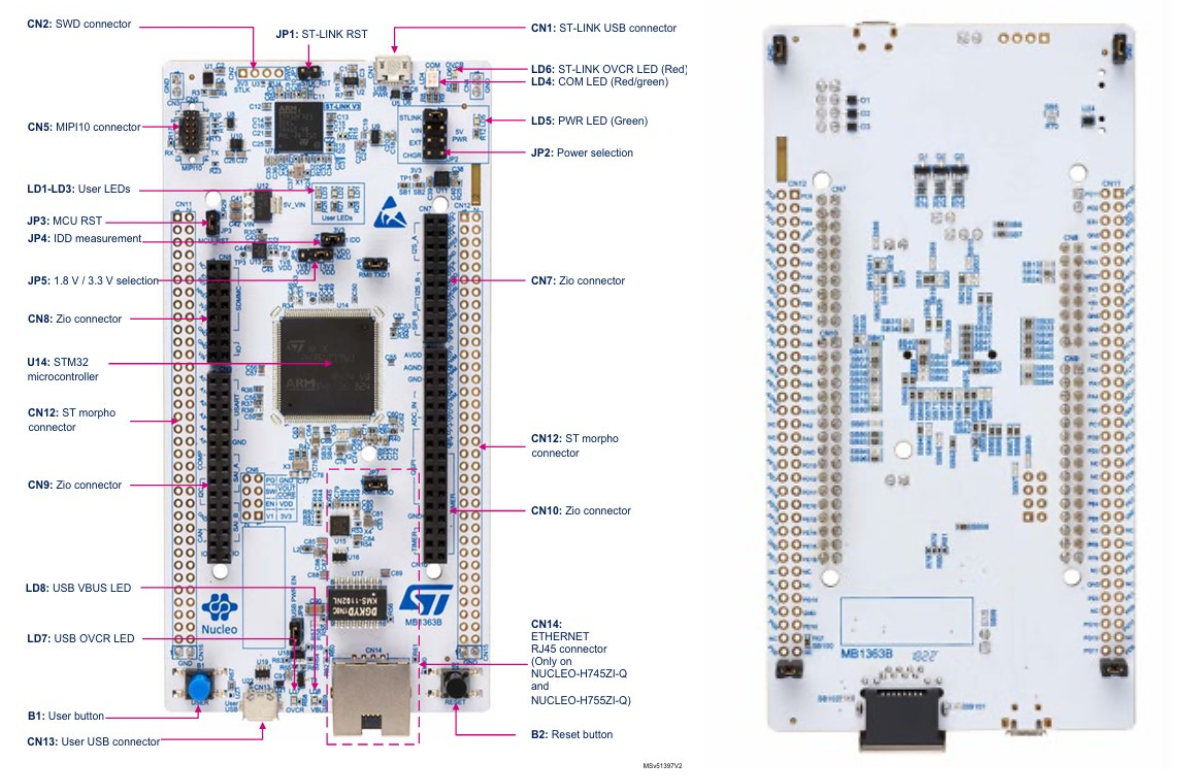
\includegraphics[width=0.7\textwidth]{images/SchedaSTM.png} 
    \captionsetup{labelsep=none}
    \caption{}    \label{fig:telaio}
\end{figure}

\section{Motore DC Reely 550er}
La trazione del veicolo viene garantita da un motore collegato alla trasmissione dello chassis.
\begin{figure}[H]
    \centering
    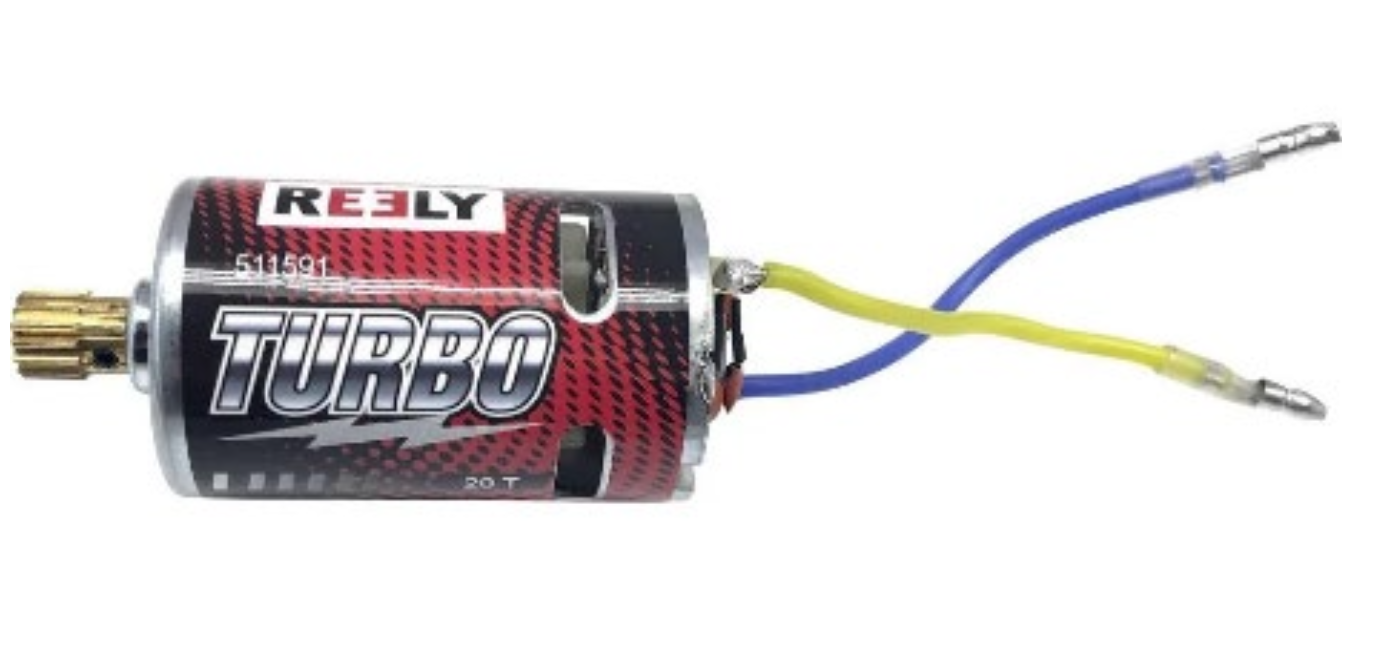
\includegraphics[width=0.5\textwidth]{images/Motore} 
    \captionsetup{labelsep=none}
    \caption{}    
    \label{fig:telaio}
\end{figure}
\noindent In particolare, viene utilizzato un motore  DC a collettore con le seguenti caratteristiche:
\begin{table}[H]
    \centering
    \label{tab:specifiche_motore}
    \vspace{0.2cm} 
    \renewcommand{\arraystretch}{1.3} 
    \begin{tabular}{@{} l c @{}}
        \toprule
        \textbf{Parametro} & \textbf{Valore} \\
        \midrule
        Tensione nominale & 4.8 -- 12 VDC \\
        Velocità di rotazione & 1000 -- 18000 RPM \\
        Coppia & 100 -- 900 g$\cdot$cm \\
        Diametro albero & 3.175 mm \\
        \bottomrule
    \end{tabular}
\end{table}

\section{Driver Motore Cytron MD10C R3}
Il motore viene controllato tramite modulazione PWM attraverso il driver MD10C-R3.
In particolare, il controllo del motore attraverso questo driver avviene tramite due segnali: 
 \begin{itemize}
\item \textbf{DIR:} controllo del verso di rotazione (Segnale digitale alto/basso) 
 \item \textbf{PWM:} controllo della velocità di rotazione (segnale PWM)
 \end{itemize}
\begin{figure}[H]
    \centering
    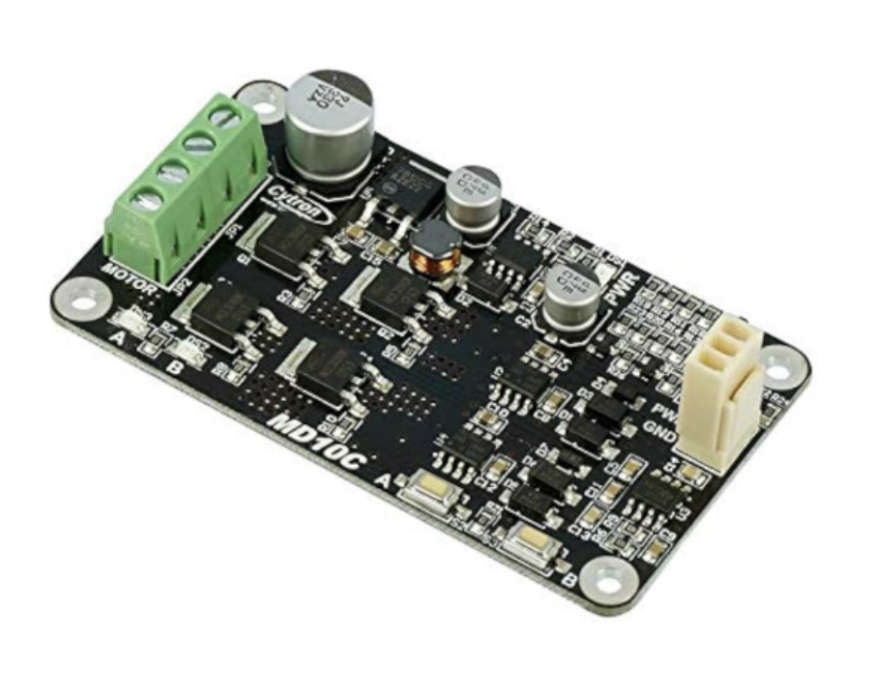
\includegraphics[width=0.5\textwidth]{images/Driver} 
    \captionsetup{labelsep=none}
    \caption{}
    \label{fig:telaio}
\end{figure}

\section{Encoder incrementale CUI Devices AMT102}
Inoltre, per effettuare il controllo del motore in velocità è necessario avere un feedback sulla velocità del motore stesso: ciò è stato reso possibile montando un encoder sull’asse posteriore del motore. In particolare, è stato utilizzato un encoder rotativo incrementale modello AMT102.
\begin{figure}[H]
    \centering
    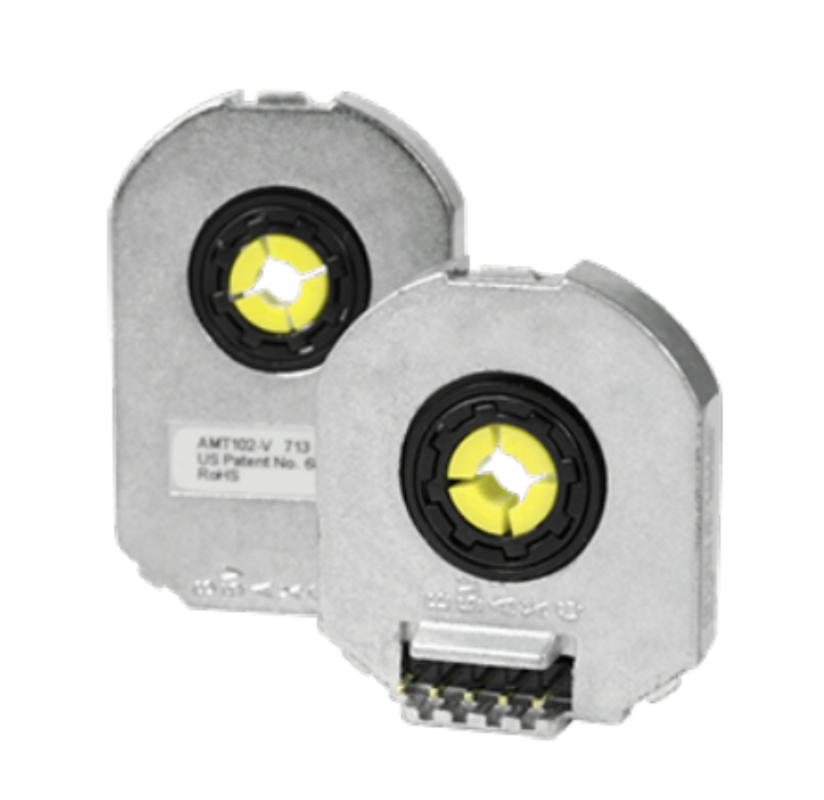
\includegraphics[width=0.4\textwidth]{images/Encoder} 
    \captionsetup{labelsep=none}
    \caption{}
    \label{fig:telaio}
\end{figure}

\section{Servomotore Miuzei MS24}
Per operare il meccanismo di sterzo del veicolo è stato impiegato un servo motore in grado di regolare il movimento angolare in modo molto preciso e proprio per
questo viene comunemente utilizzato in diverse apparecchiature elettroniche e applicazioni
che richiedono un controllo di posizione accurato.
\begin{figure}[H]
    \centering
    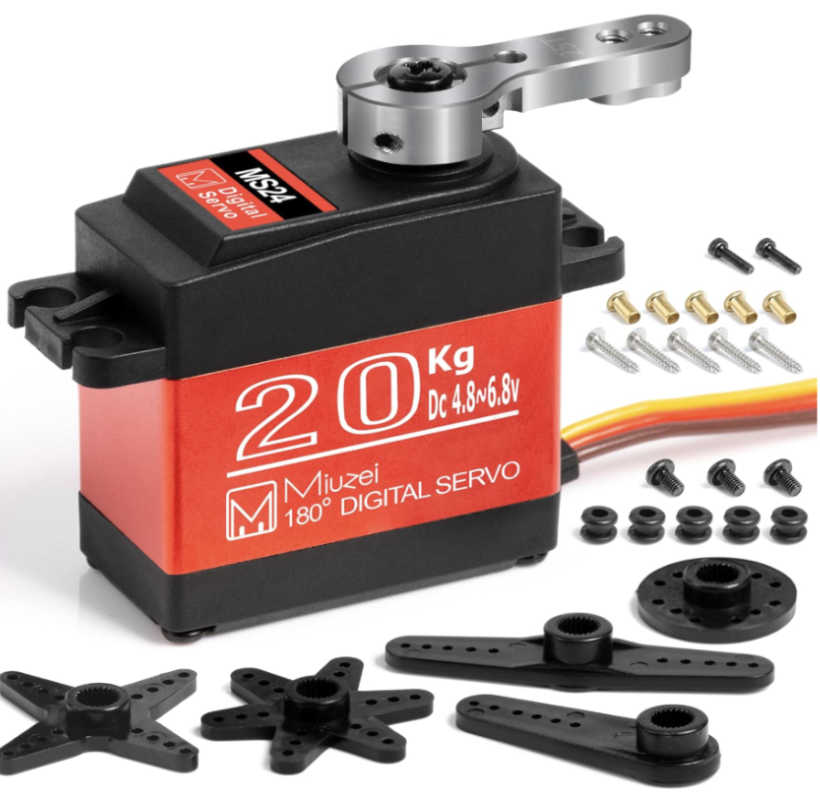
\includegraphics[width=0.4\textwidth]{images/Servo} 
    \captionsetup{labelsep=none}
    \caption{}
    \label{fig:telaio}
\end{figure}
\noindent Il dispositivo è controllato mediante un segnale PWM fornito in ingresso, calcolato dagli
algoritmi di controllo implementati sul microcontrollore.

\section{Alimentazione}
Il sistema è composto da numerose componenti, che non operano tutte alla stessa tensione.
Per questo motivo è stato necessario utilizzare dei convertitori DC-DC  XL4015, così da garantire le alimentazioni necessarie.
\begin{figure}[H]
    \centering
    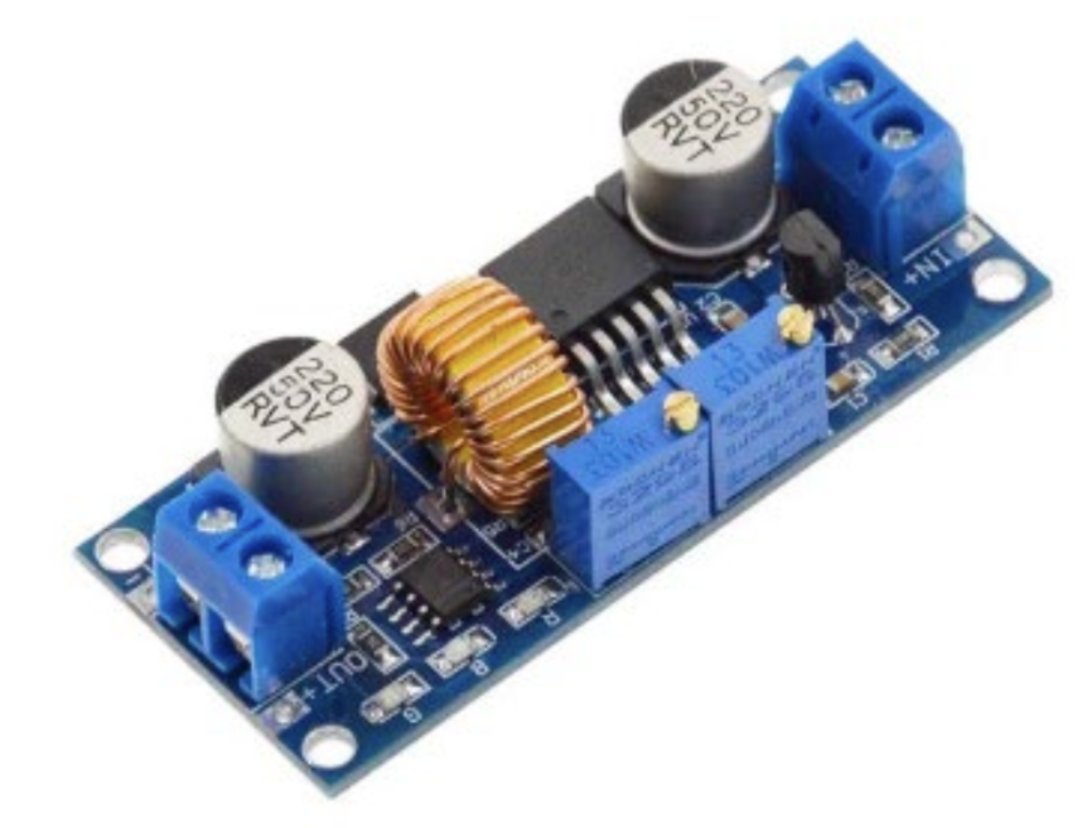
\includegraphics[width=0.4\textwidth]{images/Alimentazione} 
    \captionsetup{labelsep=none}
    \caption{}
    \label{fig:telaio}
\end{figure}

\subsection{Batteria ai polimeri di litio}
\noindent Il sistema è alimentato da una batteria ai polimeri di litio (LiPo) 2S (2 celle) con una tensione
nominale di 7.4V e una capacità di 5500 mAh, in grado di erogare una corrente di 5.5A per la durata di un’ora, garantendo una corretta alimentazione avendo una discreta autonomia.
\begin{figure}[H]
    \centering
    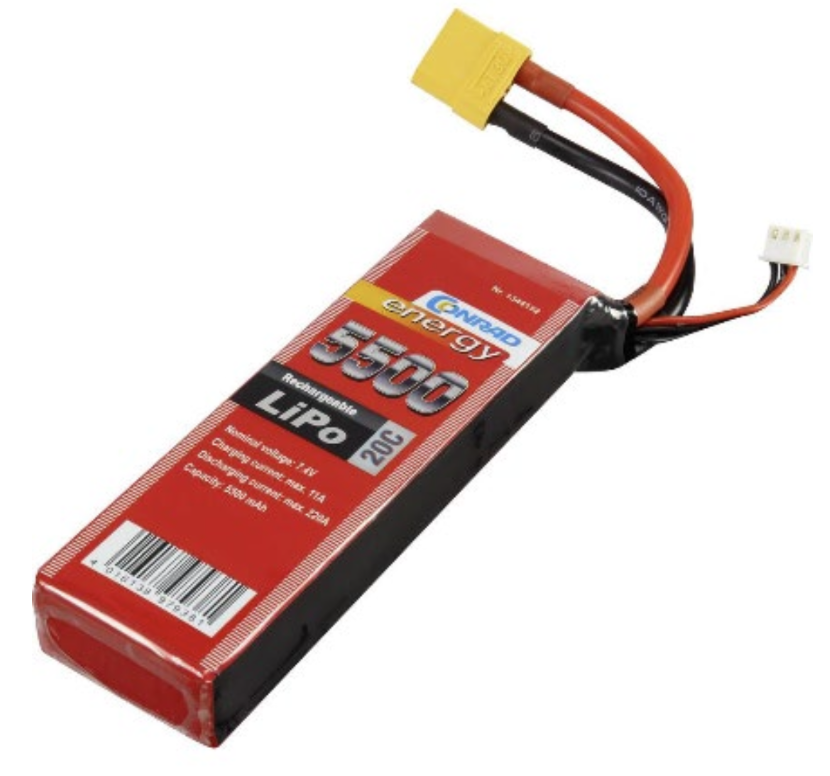
\includegraphics[width=0.4\textwidth]{images/Batteria} 
    \captionsetup{labelsep=none}
    \caption{}
    \label{fig:telaio}
\end{figure}

\section{Inertial Measurement Unit}
L’IMU è un dispositivo che misura l’accelerazione, la velocità angolare e talvolta anche il campo magnetico. Solitamente integra un accelerometro, un giroscopio e un magnetometro, ognuno avente 3 assi (in questa configurazione l’IMU si dice a 9 gradi di libertà, 9DOF). Tali misure sono di fondamentale importanza per applicazioni in cui è richiesta la navigazione e il controllo di veicoli o in altri dispositivi mobili. L’IMU scelto per questa applicazione è il BNO055 prodotto dalla Bosch Sensortech.
È caratterizzato dall’inclusione di un microcontrollere a 32 bit con
algoritmi di sensor fusion integrati, che combinano i dati grezzi dei sensori per fornire
informazioni precise su orientamento, accelerazione e rotazione dell’unità.
Il BNO055 può comunicare tramite UART o I2C.
\begin{figure}[H]
    \centering
    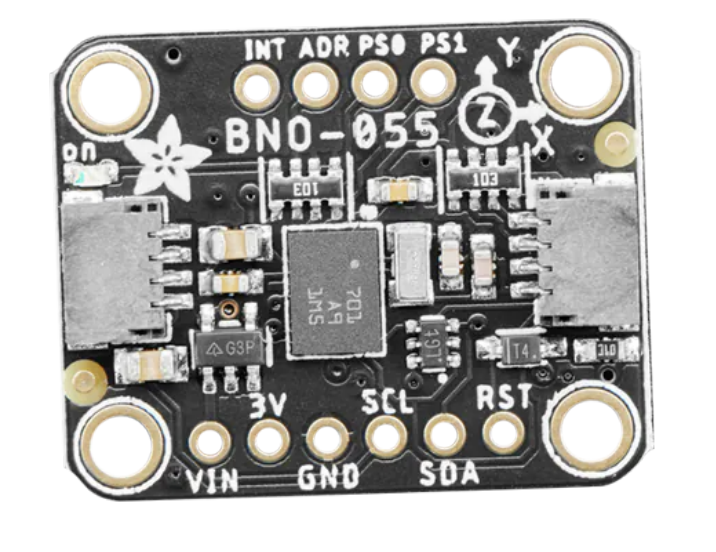
\includegraphics[width=0.4\textwidth]{images/Imu} 
    \captionsetup{labelsep=none}
    \caption{}
    \label{fig:telaio}
\end{figure}

\section{Radiocomando e Ricevitore Microzone}
Il radiocomando utilizzato per inviare segnali PWM al fine di controllare la macchinina con
un remote controller è il “Microzone 6CH Remote Transmitter Receiver System for
Drones/Quadcopters” modello: “MC6C”.
\begin{figure}[H]
    \centering
    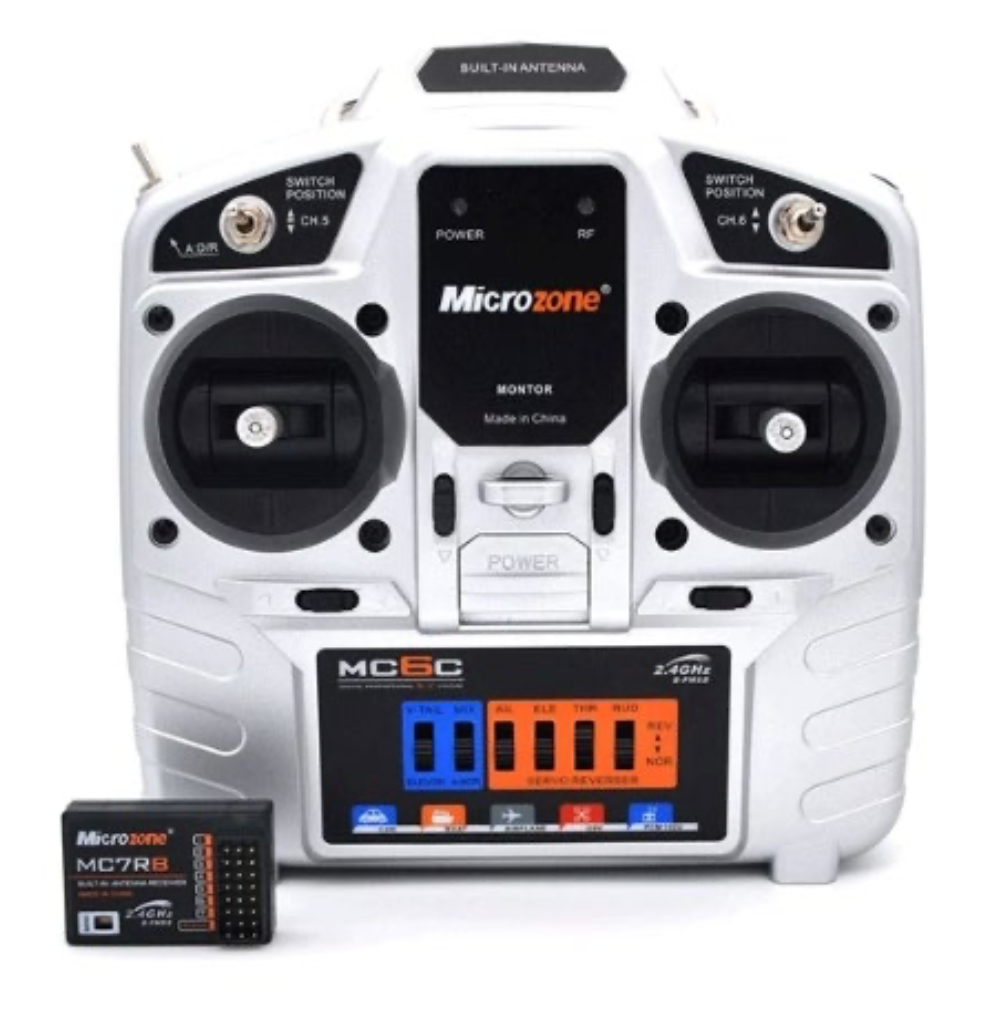
\includegraphics[width=0.4\textwidth]{images/Radiocomando} 
    \captionsetup{labelsep=none}
    \caption{}
    \label{fig:telaio}
\end{figure}
\noindent Il radiocomando dispone di sei canali e la banda va dai 2,401 GHz a 2,479 GHz. La distanza
massima di controllo è di 800m e utilizza 4 batterie xAA. Il radiocomando è inoltre dotato di
ricevitore e trasmettitore che hanno le seguenti caratteristiche:
\begin{table}[H]
    \centering
    \caption{Caratteristiche del trasmettitore}
    \label{tab:Trasmettitore}
    \vspace{0.2cm} 
    \renewcommand{\arraystretch}{1.3} 
    \begin{tabular}{@{} p{6.5cm} >{\centering\arraybackslash}p{4.5cm} @{}}
        \toprule
        \textbf{Caratteristiche} & \textbf{Valori} \\
        \midrule
        Potenza di trasmissione & $\leq$ 70 mW \\
        Range per il controllo  & 800 m \\
        Tensione (DC)           & +6 V \\
        Peso                    & 550 g \\
        Modalità di modulazione & FHSS \\
        \bottomrule
    \end{tabular}
\end{table}

\begin{table}[H]
    \centering
    \caption{Caratteristiche del ricevitore}
    \label{tab:Ricevitore}
    \vspace{0.2cm} 
    \renewcommand{\arraystretch}{1.3} 
    \begin{tabular}{@{} p{6.5cm} >{\centering\arraybackslash}p{4.5cm} @{}}
        \toprule
        \textbf{Caratteristiche} & \textbf{Valori} \\
        \midrule
        Banda di frequenza & 2.400 -- 2.483 GHz \\
        Distanza lineare & $>$ 800 m \\
        Tensione di alimentazione (DC) & 4,5 -- 6 V \\
        Tipo di segnale & PWM / SBUS \\
        Antenna & Integrata nel ricevitore \\
        Dimensioni & 45 $\times$ 45 $\times$ 10 mm \\
        Peso & 9,6 g \\
        \bottomrule
    \end{tabular}
\end{table}

\subsection{Funzionamento}
Il trasmettitore e il ricevitore comunicano tramite onde radio, le quali fungono da vettore per le istruzioni di comando generate dal pilota. Il modulo ricevitore svolge un ruolo cruciale in questa architettura: elabora i pacchetti radio in ingresso e genera in uscita un segnale PWM indipendente per ciascun canale. La variazione del \textit{Duty Cycle} di questi segnali traduce proporzionalmente i movimenti fisici eseguiti sul radiocomando in dati quantificabili dal microcontrollore.
\begin{figure}[H]
    \centering
    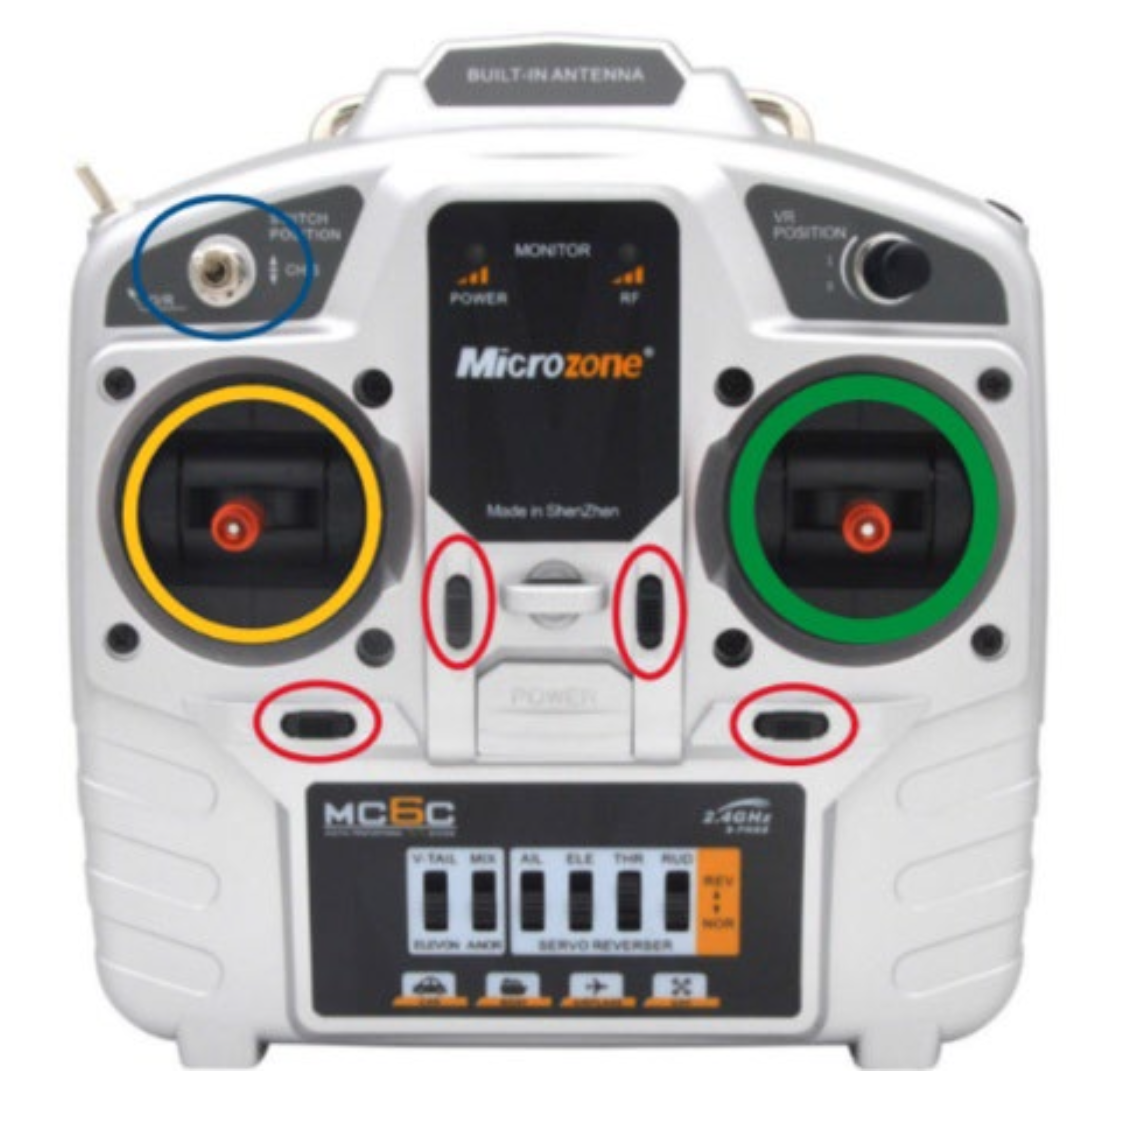
\includegraphics[width=0.4\textwidth]{images/RadiocomandoFunz} 
    \captionsetup{labelsep=none}
    \caption{}
    \label{fig:telaio}
\end{figure}
In fase di configurazione, la gestione della dinamica del veicolo è stata mappata in modo strategico su specifiche levette:

\begin{itemize}
    \item \textbf{Controllo trazione (cerchio verde):} La leva di destra è dedicata alla velocità longitudinale. Il suo azionamento lungo l'asse verticale permette di regolare la potenza erogata e far avanzare o retrocedere il veicolo.
    
    \item \textbf{Controllo sterzo (cerchio giallo):} La leva di sinistra è deputata alla gestione dell'angolo di sterzata. Questa specifica scelta di \textit{mapping} ergonomico è stata fatta perché spingere la leva orizzontalmente (a destra o a sinistra) emula in modo molto più naturale e intuitivo il movimento direzionale delle ruote. Tale spostamento trasversale si traduce direttamente nella variazione del segnale PWM inviato al servomotore.
    
    \item \textbf{Armamento motore (cerchio blu):} Lo \textit{switch} a tre scatti, situato in alto a sinistra, funge da sistema di sicurezza (abilitazione hardware) per l'armamento del motore. Nelle posizioni estreme (completamente in alto o in basso) il motore è forzatamente spento e disarmato, mentre posizionando la levetta al centro il sistema viene armato ed è pronto a ricevere potenza dalla trazione.
    
    \item \textbf{Regolazione fine (cerchi rossi):} Infine, i \textit{trimmer} fisici consentono di applicare un \textit{offset} ai segnali. Questi pulsanti traslano leggermente l'intervallo di base del \textit{Duty Cycle} sui primi quattro canali, rivelandosi essenziali per calibrare elettronicamente lo "zero" meccanico dello sterzo e del motore senza dover intervenire via software.
\end{itemize}

 \subsection{ Canali del ricevitore}
Il ricevitore è dotato di sei canali che permettono di gestire i segnali generati
dallo spostamento delle varie levette. La seguente tabella riporta la relazione tra canali e leve.
\begin{table}[H]
    \centering
    \caption{Mappatura dei canali del radiocomando}
    \label{tab:canali_radiocomando}
    \vspace{0.2cm} 
    \renewcommand{\arraystretch}{1.3} 
    \begin{tabular}{@{} l l @{}}
        \toprule
        \textbf{Canale} & \textbf{Leva del radiocomando} \\
        \midrule
        Channel 1 & Leva destra orizzontale \\
        Channel 2 & Leva destra verticale \\
        Channel 3 & Leva sinistra verticale \\
        Channel 4 & Leva sinistra orizzontale \\
        Channel 5 & Levetta in alto a sinistra (a 3 posizioni) \\
        Channel 6 & Rotella in alto a destra \\
        \bottomrule
    \end{tabular}
\end{table}
Per la realizzazione del progetto sono stati utilizzati solo i canali 2 e 4 per le levette.

\section{Schema dei collegamenti}
La Figura \ref{fig:schema} illustra lo schema generale dei collegamenti elettrici e di segnale che costituiscono l'architettura hardware del prototipo. Il sistema è centralizzato attorno alla scheda di sviluppo STM32, la quale funge da nodo principale per l'elaborazione logica, l'acquisizione dei dati e il controllo degli attuatori. 

\begin{figure}[H]
\centering
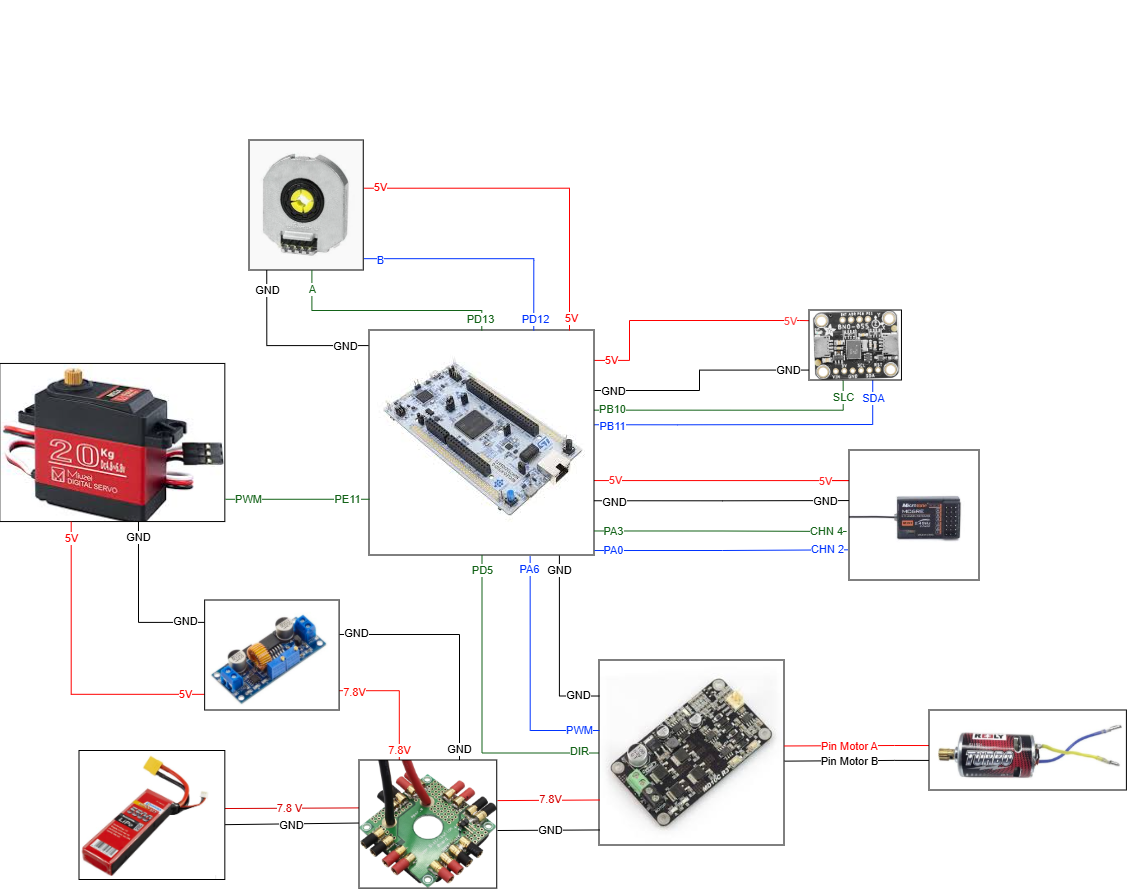
\includegraphics[width=0.8\textwidth,keepaspectratio]{images/diagramma_componenti.png}
\caption{Schema dei collegamenti}
\label{fig:schema}
\end{figure}


\chapter{Software}
Il presente capitolo descrive gli applicativi software impiegati per lo sviluppo del progetto. L'utilizzo di tali strumenti ha consentito la programmazione del microcontrollore e la successiva implementazione degli algoritmi di controllo necessari al funzionamento dinamico del veicolo. Inoltre, l'infrastruttura software si è rivelata un supporto fondamentale durante la fase di \textit{testing}, permettendo l'acquisizione e la visualizzazione in tempo reale dei parametri di telemetria e dei grafici di risposta del sistema.

\subsection{STM32CubeIDE}
Il firmware per la scheda STM32H755ZI-Q è stato interamente sviluppato in linguaggio C avvalendosi di STM32CubeIDE, l'ambiente di sviluppo integrato ufficiale di STMicroelectronics. Quest'ultimo mette a disposizione un'avanzata interfaccia grafica che, tramite un file di configurazione con estensione \texttt{.ioc}, permette di inizializzare l'hardware del microcontrollore in modo rapido e intuitivo. Tra le principali impostazioni gestite figurano:
\begin{itemize}
    \item Configurazione dell'albero di \textit{clock} del sistema;
    \item Assegnazione e configurazione dei pin di input/output (GPIO);
    \item Setup dei Timer hardware (es. per la generazione del PWM e la lettura dell'encoder);
    \item Inizializzazione delle interfacce di comunicazione (UART, I$^2$C, SPI).
\end{itemize}

\noindent Una volta ultimata la configurazione grafica, l'IDE provvede alla generazione automatica del codice C di base, fornendo un'architettura software pre-inizializzata su cui lo sviluppatore può procedere direttamente all'implementazione della logica di controllo.

\subsection{MATLAB}
MATLAB, ambiente di calcolo numerico e linguaggio di programmazione sviluppato da MathWorks, è uno strumento ampiamente impiegato in ambito ingegneristico per l'analisi dei dati, lo sviluppo di algoritmi, la simulazione di sistemi di controllo e l'elaborazione dei segnali. Il software si distingue per una sintassi intuitiva, un'architettura ottimizzata per la gestione di matrici e vettori, e la disponibilità di numerosi \textit{toolbox} settoriali, uniti a potenti interfacce per la visualizzazione grafica in 2D e 3D.
All'interno di questo progetto, le funzionalità di \textit{plotting} di MATLAB sono state impiegate specificamente per l'acquisizione e la visualizzazione dei dati in tempo reale (\textit{real-time}), fornendo un prezioso supporto visivo per il monitoraggio delle variabili in gioco e la validazione del comportamento dinamico del veicolo.

\subsection{Acquisizione dati via Terminale}
Per la cattura e la verifica preliminare dei dati telemetrici inviati dal microcontrollore, ci si è avvalsi del terminale nativo di macOS in esecuzione su un MacBook Pro M2. Sfruttando la comunicazione seriale (UART via USB) tra la scheda STM32 e il computer, l'interfaccia a riga di comando ha permesso di monitorare e registrare il flusso continuo di dati grezzi in uscita. Questa procedura si è rivelata uno step di \textit{debug} cruciale: ha consentito di verificare l'integrità, la frequenza e la corretta formattazione dei pacchetti dati (come i conteggi dell'encoder o l'errore del PID) prima che questi venissero acquisiti ed elaborati dall'ambiente MATLAB per il \textit{plotting} in tempo reale.

\chapter{Implementazione del firmware}
In questo capitolo verranno analizzati gli algoritmi di controllo sviluppati sul microcontrollore
dal punto di vista della loro implementazione. La trattazione sarà divisa in quattro sezioni, la
prima fornirà una descrizione generale della struttura del codice, mentre le successive
riguarderanno ognuna un aspetto fondamentale del moto del veicolo: ossia il controllo del
radiocomando, della trazione e dello sterzo.
\section{Diagramma di flusso}
Si descrivere in maniera complessiva la logica del sistema attraverso il successivo
diagramma di flusso \ref{fig:diagramma}: 


\begin{figure}[H]
\centering
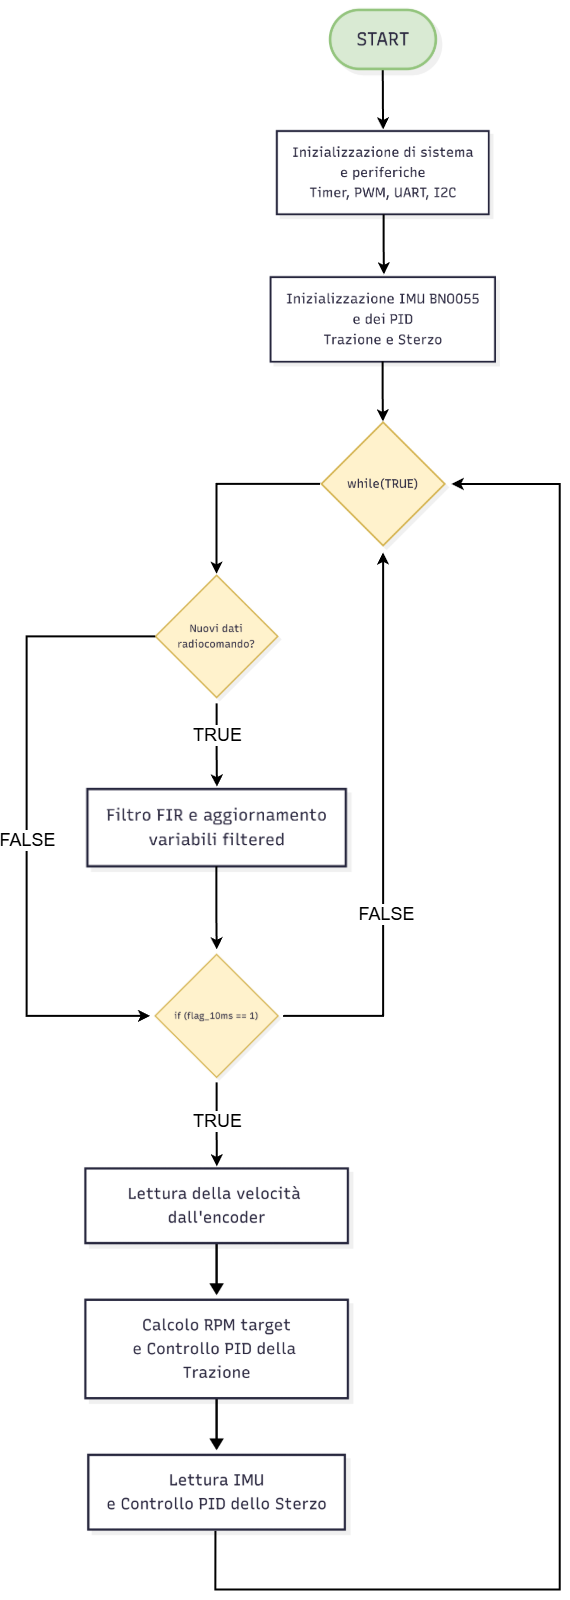
\includegraphics[width=\textwidth, height=0.85\textheight, keepaspectratio]{images/diagramma_di_flusso.png}
\caption{Diagramma di flusso del codice sviluppato}
\label{fig:diagramma}
\end{figure}

Si evidenzia come il flusso di esecuzione delle istruzioni del codice inizi con una fase preliminare di setup, in cui vengono inizializzate le periferiche di sistema (Timer, PWM, UART, I2C) e configurati i componenti essenziali, ovvero l'unità inerziale (IMU BNO055) e i due regolatori PID per il controllo della trazione e dello sterzo. Successivamente, il programma entra in un 
ciclo di esecuzione infinito, rappresentato dal blocco “while(TRUE)”. 
All'interno di questo ciclo, il flusso operativo dipende dall'esito di due blocchi condizionali principali. Il primo verifica costantemente la ricezione di nuovi comandi impartiti tramite il radiocomando. Quando questa condizione è verificata (TRUE), i segnali grezzi in ingresso vengono elaborati attraverso un filtro FIR (Finite Impulse Response), 
al fine di smorzarne le oscillazioni, e vengono aggiornate le rispettive variabili filtrate che rappresentano il setpoint imposto dal pilota. Nel caso in cui non vi siano nuovi dati (FALSE), l'algoritmo salta l'elaborazione del filtro.
Il flusso prosegue poi verso la seconda condizione, che rappresenta il cuore del sistema di controllo in tempo reale: la verifica della variabile temporale “flag\_10ms”. Se tale variabile assume il valore 1 (TRUE), significa che è trascorso il periodo di campionamento prefissato di 10 millisecondi. In questa occorrenza, il sistema esegue in stretta 
sequenza le operazioni necessarie per il movimento del veicolo: procede prima con la lettura della velocità attuale dall'encoder, il calcolo degli RPM target e l'esecuzione del controllo PID della trazione; successivamente effettua la lettura del tasso di imbardata reale dall'IMU per alimentare il controllo PID dello sterzo. 
Al termine di queste operazioni, o nel caso in cui il periodo di 10ms non sia ancora trascorso (FALSE), il flusso ritorna all'inizio del ciclo per ripetere le verifiche. Tutti gli algoritmi utilizzati sono stati sviluppati mediante linguaggio C e l’ambiente di sviluppo STM32CubeIDE.

\section{Implementazione relativa al radiocomando}
L'implementazione relativa al radiocomando rappresenta il fulcro di questa relazione:
l’obiettivo del progetto è infatti proprio quello di gestire la comunicazione tra radiocomando
e microcontrollore, al fine di gestire il moto del veicolo (trazione e sterzo).

\subsection{Impostazioni iniziali timers e calcolo preliminare di frequenza e duty}
In questa sottosezione si riportano le impostazioni inziali dei Timers e il codice utilizzato per
l’acquisizione dei primi valori di frequenza e duty fondamentali per le fasi di implementazione
successive.
Inizialmente si è analizzato il segnale PWM restituito da ogni canale del ricevitore. Per
ottenere la frequenza ed il duty cycle tutti i canali, è stato utilizzato un interrupt in modalità
InputCapture che consente di studiare un segnale preso come input, generato appunto dal
ricevitore. Tramite la configurazione nel file “.ioc” di questo interrupt, è necessario specificare
la “Polarity Section”, ovvero a quale evento del segnale si è interessati: “Rising Edge” (fronte
di salita), “Falling Edge” (fronte di discesa), “Both Edges” (fronte di salita e di discesa).
Grazie a quanto appreso da relazioni precedenti in cui si era utilizzato un oscilloscopio, si è a
conoscenza del fatto che tutti i segnali sono sincronizzati tra loro, ovvero hanno stessa
frequenza e non sono sfasati tra loro. Questa osservazione sarà utile in un secondo momento.

\subsubsection{Impostazioni timer}
I timer permettono di misurare il tempo e quindi di ottenere i valori desiderati dalla ricevente. Per l'utilizzo dell'Input Capture (sfruttando i canali PA0 e PA3 del TIM5) si è deciso di utilizzare un timer con un clock di 64 MHz, che viene diviso dal "Prescaler". Poiché a livello hardware il microcontrollore somma sempre 1 al valore del registro, per ottenere un clock effettivo di 1 MHz il parametro è stato settato a 63, calcolato mediante la formula $PSC = \frac{64.000.000}{1.000.000} - 1$.

Inoltre, poiché la frequenza minima leggibile è data da $\frac{TIMCLOCK}{COUNTERPERIOD}$, si è deciso di lasciare il "Counter Period" al massimo, ovvero 0xffffffff (corrispondente a 4294967295) essendo il TIM5 un timer a 32 bit.
    \begin{figure}[H]
\centering
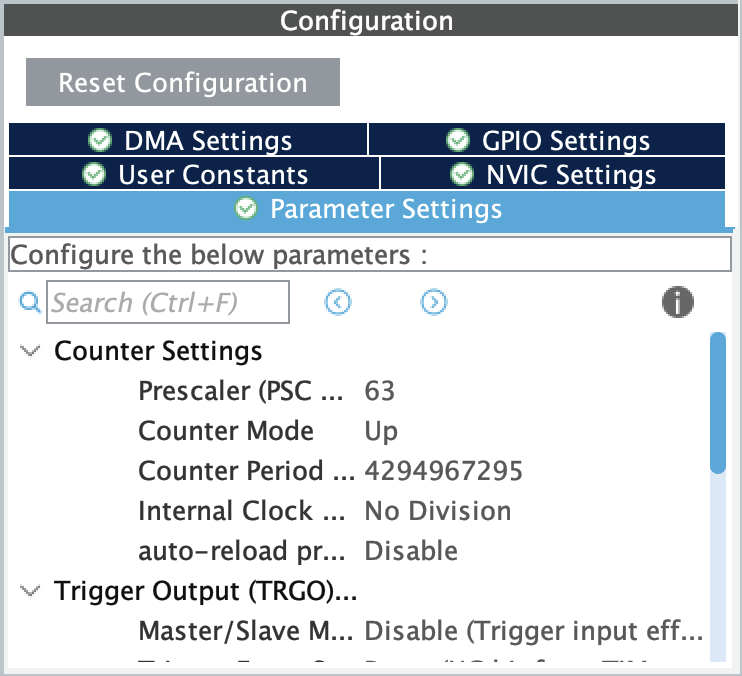
\includegraphics[width=0.7\textwidth,keepaspectratio]{images/impostazioni_timer.png}
\caption{Impostazioni timer}
\label{fig:impostazioni_timer}
\end{figure}
\subsubsection{Acquisizione del segnale PWM}
Il segnale PWM in uscita dal ricevitore del radiocomando presenta una frequenza fissa (tipicamente 50 Hz, pari a un periodo di 20 ms). Pertanto, il calcolo della frequenza risulta irrilevante ai fini del controllo dinamico del veicolo. L'informazione vitale legata al comando impartito dal pilota risiede unicamente nella larghezza dell'impulso alto ($T_{on}$), che varia proporzionalmente al movimento delle levette in un intervallo tipicamente compreso tra 1000 $\mu$s e 2000 $\mu$s.

Per acquisire direttamente questo dato vitale, si è configurato il parametro ``Polarity Selection'' su ``Both Edges'' all'interno dell'ambiente di sviluppo, discostandosi da un approccio basato sul solo fronte di salita. 

\begin{figure}[H]
\centering
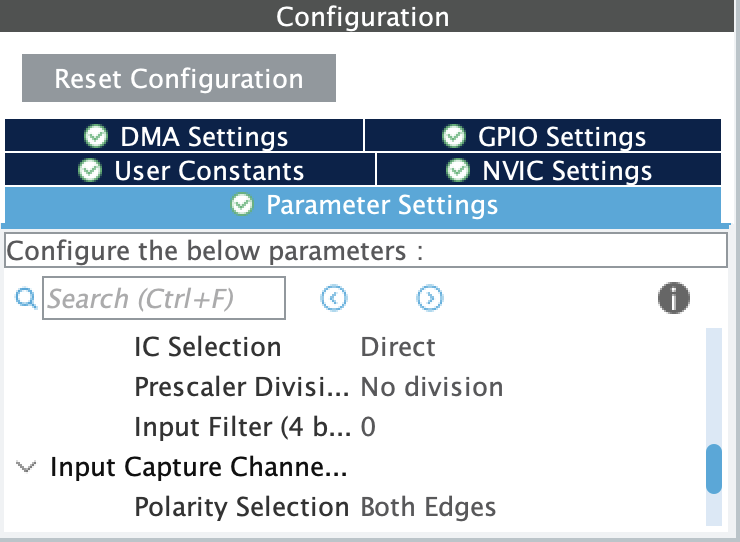
\includegraphics[width=0.7\textwidth,keepaspectratio]{images/BothEdges.png} 
\caption{Configurazione Polarity Selection su Both Edges}
\label{fig:polarity_both}
\end{figure}

La logica di acquisizione è gestita all'interno della funzione di callback \texttt{HAL\_TIM\_IC\_CaptureCallback}. Tramite l'ausilio di flag di stato (come \texttt{Is\_First\_Captured\_Steering}), il sistema salva il valore del contatore hardware al verificarsi del fronte di salita, commutando contestualmente la sensibilità del canale sul fronte opposto. Al successivo fronte di discesa, il contatore viene letto nuovamente per poterne calcolare la differenza temporale. 

Poiché il timer opera con un clock effettivo di 1 MHz, la differenza algebrica tra le due letture restituisce la durata dell'impulso espressa direttamente in microsecondi. Tale valore viene salvato nelle variabili globali (\texttt{steering\_us} e \texttt{throttle\_us}) per essere impiegato come setpoint, a patto che superi il controllo di sicurezza implementato per scartare letture anomale esterne al range nominale (600--2400 $\mu$s).

\begin{lstlisting}[language=Cpp, caption="Codice per la lettura del segnale PWM tramite Input Capture"]
void HAL_TIM_IC_CaptureCallback(TIM_HandleTypeDef *htim)
{
    // STERZO -> PA3 (TIM5 CH4)
    if (htim->Instance == TIM5 && htim->Channel == HAL_TIM_ACTIVE_CHANNEL_4)
    {
        static uint32_t ic_val1_s = 0;
        uint32_t ic_val2_s = 0;
        uint32_t diff_steering = 0;

        if (Is_First_Captured_Steering == 0)
        {
            ic_val1_s = HAL_TIM_ReadCapturedValue(htim, TIM_CHANNEL_4);
            Is_First_Captured_Steering = 1;
            __HAL_TIM_SET_CAPTUREPOLARITY(htim, TIM_CHANNEL_4, TIM_INPUTCHANNELPOLARITY_FALLING);
        }
        else
        {
            ic_val2_s = HAL_TIM_ReadCapturedValue(htim, TIM_CHANNEL_4);

            if (ic_val2_s > ic_val1_s)
                diff_steering = ic_val2_s - ic_val1_s;
            else
                diff_steering = (0xFFFFFFFF - ic_val1_s) + ic_val2_s;

            // Per lo sterzo FIR
            if (diff_steering > 600 && diff_steering < 2400) {
                steering_us = diff_steering;
                new_rc_steering = 1;
            }

            Is_First_Captured_Steering = 0;
            __HAL_TIM_SET_CAPTUREPOLARITY(htim, TIM_CHANNEL_4, TIM_INPUTCHANNELPOLARITY_RISING);
        }
    }

    // Trazione -> PA0 (TIM5 CH1)
    if (htim->Instance == TIM5 && htim->Channel == HAL_TIM_ACTIVE_CHANNEL_1)
    {
        static uint32_t ic_val1_t = 0;
        uint32_t ic_val2_t = 0;
        uint32_t diff_throttle = 0;

        if (Is_First_Captured_Throttle == 0)
        {
            ic_val1_t = HAL_TIM_ReadCapturedValue(htim, TIM_CHANNEL_1);
            Is_First_Captured_Throttle = 1;
            __HAL_TIM_SET_CAPTUREPOLARITY(htim, TIM_CHANNEL_1, TIM_INPUTCHANNELPOLARITY_FALLING);
        }
        else
        {
            ic_val2_t = HAL_TIM_ReadCapturedValue(htim, TIM_CHANNEL_1);

            if (ic_val2_t > ic_val1_t)
                diff_throttle = ic_val2_t - ic_val1_t;
            else
                diff_throttle = (0xFFFFFFFF - ic_val1_t) + ic_val2_t;

            if (diff_throttle > 600 && diff_throttle < 2400) {
                throttle_us = diff_throttle;
                new_rc_throttle = 1;
            }

            Is_First_Captured_Throttle = 0;
            __HAL_TIM_SET_CAPTUREPOLARITY(htim, TIM_CHANNEL_1, TIM_INPUTCHANNELPOLARITY_RISING);
        }
    }
}
\end{lstlisting}

\subsubsection{Gestione degli Interrupt e ottimizzazione dei Timer}

A differenza delle classiche implementazioni hardware che prevedono l'azzeramento forzato del contatore del timer ad ogni fronte di salita (metodologia che impedisce la lettura simultanea di più canali e costringe all'utilizzo di molteplici timer), in questo progetto si è optato per un approccio software non distruttivo.

Come si evince dalla configurazione di sistema in STM32CubeMX (Figura \ref{fig:tim5_configurazione}), il timer dedicato alla decodifica (TIM5) è attivamente impiegato sui canali 1 e 4 in modalità \textit{Input Capture direct mode}, ma il suo contatore viene fatto avanzare in modo continuo (fino al suo limite massimo a 32 bit, pari a 4294967295) senza mai subire reset forzati. All'attivazione dell'interrupt, la \textit{callback} si limita a "fotografare" il valore assoluto del registro (tramite la funzione \verb|HAL_TIM_ReadCapturedValue|).

\begin{figure}[H]
\centering
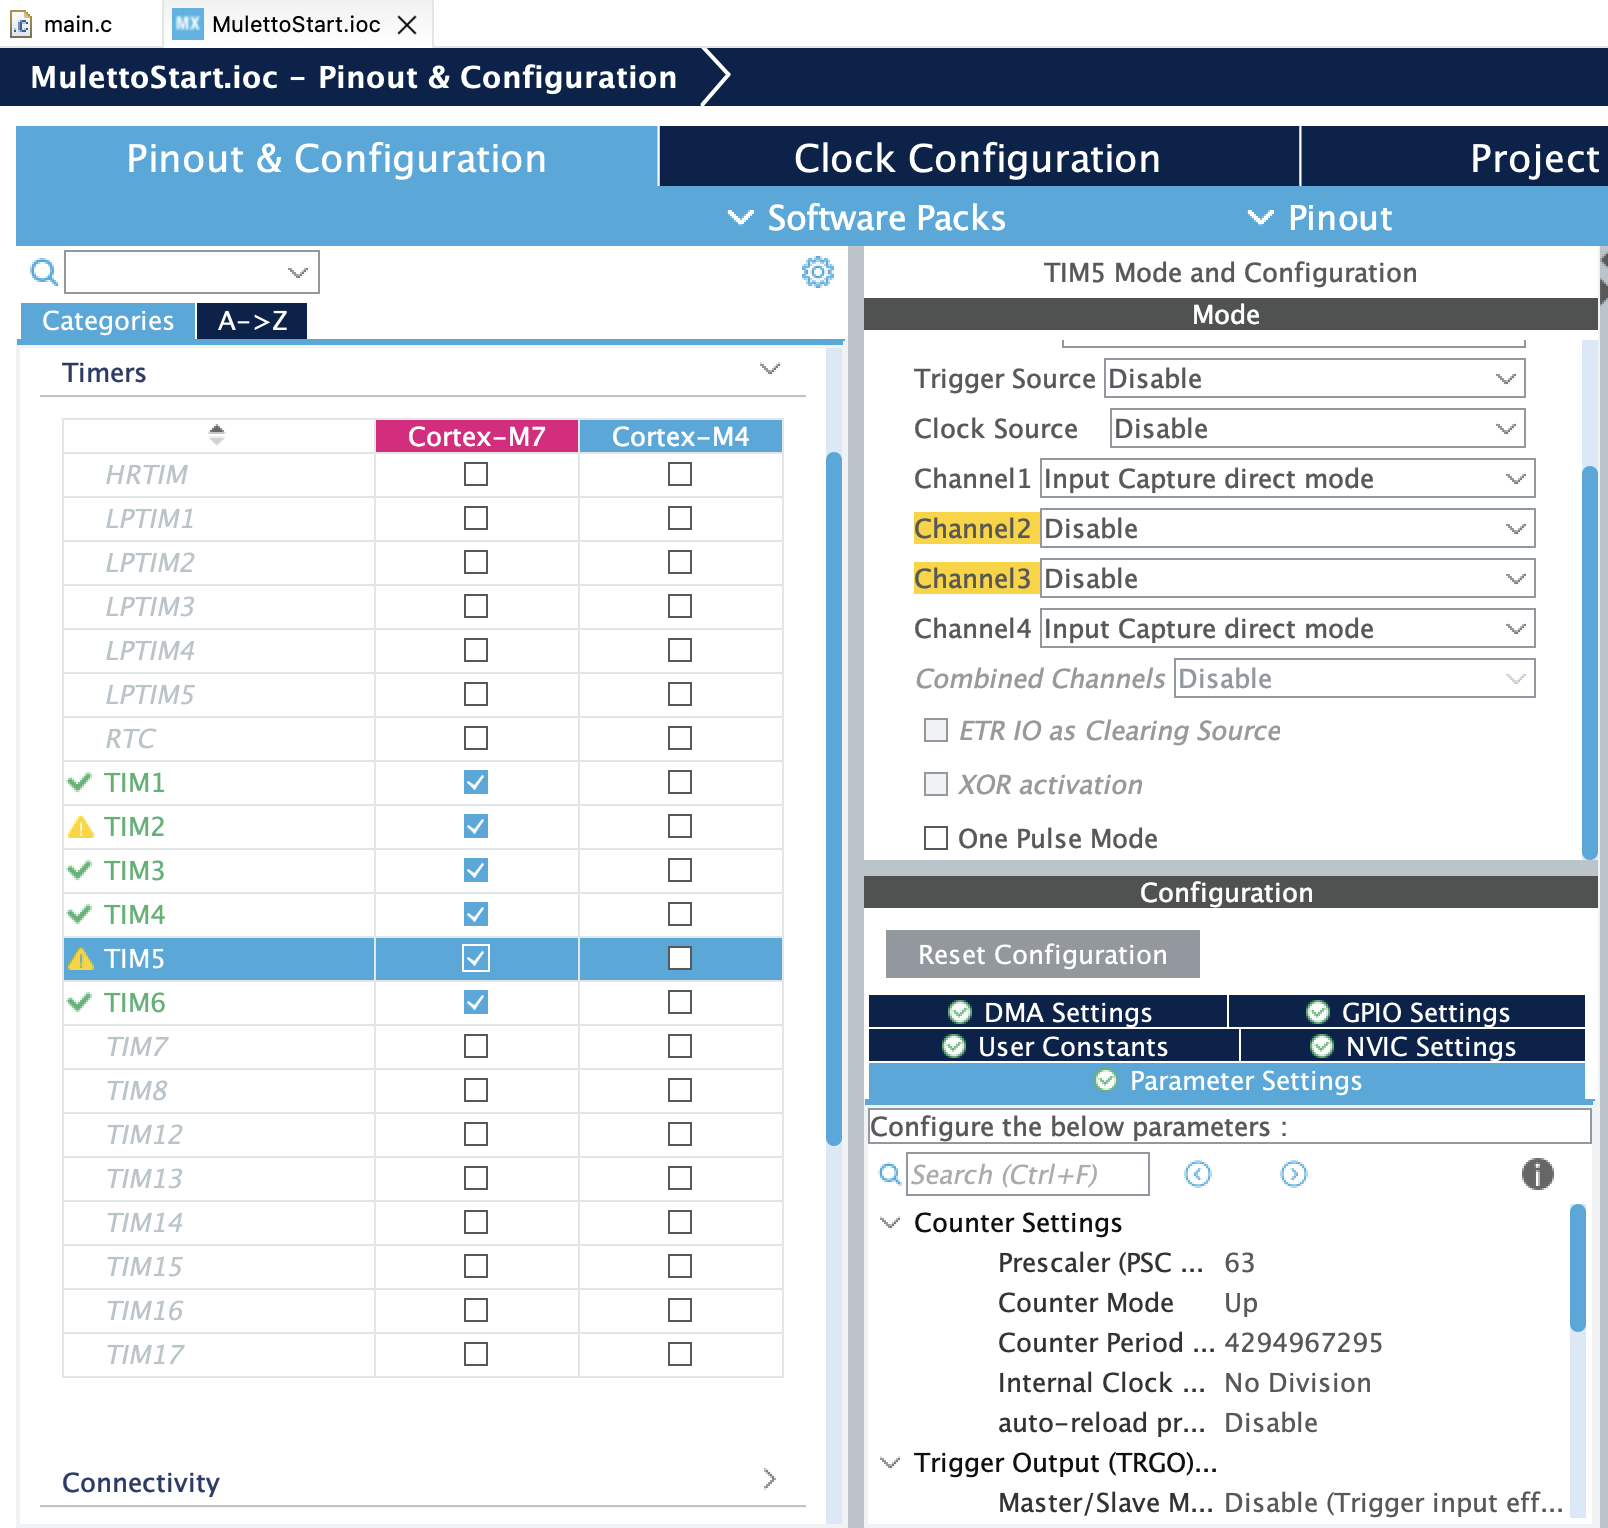
\includegraphics[width=1\textwidth,keepaspectratio]{images/Timer5_Channels.png} 
\caption{Configurazione del TIM5 con i canali 1 e 4 attivi}
\label{fig:tim5_configurazione}
\end{figure}

La durata dell'impulso viene così ricavata puramente per differenza matematica tra il timestamp di discesa e quello di salita. Per prevenire errori di calcolo nel raro caso in cui avvenga un overflow del timer proprio durante un impulso, l'algoritmo include un controllo condizionale che compensa il riavvio del conteggio sommano il complemento a due del limite massimo.

Questa architettura software garantisce numerosi vantaggi:
\begin{itemize}
    \item \textbf{Ottimizzazione delle risorse:} consente di gestire in modo totalmente asincrono e indipendente l'acquisizione dei comandi Xa e Xb utilizzando un unico timer (TIM5) e due soli canali, riducendo il carico computazionale e liberando le restanti periferiche del microcontrollore.
    \item \textbf{Assenza di interferenze:} poiché il contatore principale non viene mai azzerato, l'arrivo di un interrupt sul canale dedicato a Xb non corrompe in alcun modo il conteggio temporale in corso sul canale di Xa, garantendo una precisione assoluta su entrambi i segnali in ingresso.
    \item \textbf{Flessibilità della polarità:} la commutazione dinamica della polarità (da \textit{Falling} a \textit{Rising} e viceversa) viene gestita direttamente all'interno della singola routine di interrupt.
\end{itemize}

\subsubsection{Struttura codice principale}
In questo progetto si è scelto di centralizzare l'acquisizione e il filtraggio dei comandi direttamente all'interno del file \verb|main.c|. Questa architettura riduce l'overhead delle chiamate a funzioni, ottimizzando i tempi di esecuzione per il sistema di controllo in tempo reale. Il codice si articola in tre concetti fondamentali per il trattamento dei dati:
\begin{enumerate}
    \item \textbf{Struttura dati centralizzata}\\
    Invece di utilizzare strutture separate unicamente per la lettura temporale dei segnali, lo stato globale e le cinematiche della vettura sono state incapsulate in un'unica \verb|struct| denominata \verb|vehicleData|. Questa struttura funge da raccoglitore univoco per tutte le metriche fondamentali, semplificando enormemente la gestione della memoria e il passaggio di parametri alle funzioni di controllo.

    \begin{lstlisting}[language=Cpp, caption="Definizione della struttura dati del veicolo"]
typedef struct VehicleData {
    // Trazione (Xa)
    int counts;
    int ref_count;
    int delta_count;
    float motor_speed_RPM;
    float linear_speed_m_s;
    float motor_speed_ref_RPM;
    uint8_t motor_direction_ref;

    // Sterzo (Xb)
    double yaw_rate_rad_sec;
    double yaw_rate_deg_sec;
    double yaw_rate_ref_rad_sec;
} vehicleData;
    \end{lstlisting}

    \item \textbf{Stabilizzazione e Zona Morta (Dead Band)}\\
    I potenziometri fisici presenti sui radiocomandi commerciali sono intrinsecamente soggetti a lievi fluttuazioni elettriche e rumore meccanico. Se non filtrati, tali disturbi farebbero percepire al microcontrollore un comando variabile anche quando le levette sono a riposo (centrate idealmente a 1500 $\mu$s), causando impercettibili movimenti dei motori.
    Per ovviare a questo problema, è stata implementata via software una "zona morta" di sicurezza. Come visibile nel codice, qualsiasi variazione del segnale di trazione (\textbf{Xa}) e di sterzo (\textbf{Xb}) che ricada nell'intorno del punto di neutro viene forzatamente ignorata, garantendo il perfetto arresto del veicolo e l'allineamento delle ruote anteriori.

    \begin{lstlisting}[language=Cpp, caption="Implementazione della zona morta per Xa e Xb"]
// Zona morta per la trazione (Xa)
if(throttle_filtered > 1560.0f) {
    target_dir = 1;
    target_rpm = ((throttle_filtered - 1560.0f) * MAX_TARGET_RPM) / 433.0f;
}
else if(throttle_filtered < 1440.0f) {
    target_dir = 0;
    target_rpm = ((1440.0f - throttle_filtered) * MAX_TARGET_RPM) / 449.0f;
}
else {
    target_rpm = 0.0f;
    target_dir = 0;
    pid_traction.Iterm = 0;
    pid_traction.e_old = 0;
}

// Zona morta per lo sterzo (Xb)
if (steering_filtered > 1460.0f && steering_filtered < 1560.0f) {
    pid_steering.Iterm = 0;
    pid_steering.e_old = 0;
    u_sterzo = 0.0f;
}
    \end{lstlisting}

    \item \textbf{Ciclo Infinito (Main Loop)}\\
    Tutte queste operazioni avvengono costantemente all'interno del ciclo infinito \verb|while(1)|. Qui i segnali grezzi intercettati dagli interrupt vengono passati prima attraverso un filtro FIR per regolarizzarne l'andamento, poi limitati dalle zone morte descritte in precedenza e infine mappati nei riferimenti (setpoint) da fornire agli anelli di controllo PID.
\end{enumerate}

\subsubsection{Operazioni di inizializzazione e avvio dei Timer}
L'approccio implementato per l'avvio e la configurazione del sistema all'interno del \verb|main.c| si basa su una logica del tutto asincrona e non bloccante. Le operazioni iniziali si limitano ad avviare le periferiche necessarie in sequenza, delegando l'intera logica di allineamento al fronte d'onda alla macchina a stati finiti (gestita tramite i flag software) implementata direttamente all'interno della routine di \textit{interrupt}.
In particolare, per quanto riguarda l'acquisizione dei segnali provenienti dal radiocomando (Xa per la trazione e Xb per lo sterzo), è sufficiente abilitare gli \textit{interrupt} legati all'Input Capture sui canali 1 e 4 del TIM5. Contestualmente, viene avviato il timer di base (TIM6) che scandisce il ciclo di controllo primario ogni 10 ms.
\begin{lstlisting}[language=Cpp, caption="Avvio delle periferiche hardware e del sistema di controllo"]
// Avvio del Timer per il ciclo di esecuzione a 10ms
HAL_TIM_Base_Start_IT(&htim6);
// Avvio degli interrupt di Input Capture per Xa (Trazione) e Xb (Sterzo)
HAL_TIM_IC_Start_IT(&htim5, TIM_CHANNEL_1);
HAL_TIM_IC_Start_IT(&htim5, TIM_CHANNEL_4);
// Inizializzazione delle strutture PID per trazione e sterzo
init_PID(&pid_traction, TRACTION_SAMPLING_TIME, MAX_U_TRACTION, MIN_U_TRACTION);
tune_PID(&pid_traction, KP_TRACTION, KI_TRACTION, 0);
init_PID(&pid_steering, STEERING_SAMPLING_TIME, MAX_U_STEERING, MIN_U_STEERING);
tune_PID(&pid_steering, KP_STEERING, KI_STEERING, 0);
\end{lstlisting}
Questo paradigma architetturale snellisce il codice sorgente e riduce i tempi di accensione del sistema (\textit{boot}), scongiurando inoltre il rischio di blocchi critici (\textit{deadlock}) nel caso in cui il radiocomando sia spento al momento dell'accensione del microcontrollore. Essendo privo di attese bloccanti, il flusso principale continua la sua esecuzione naturale, inizializzando i sensori (come l'IMU via I$^2$C) e posizionando le variabili di sicurezza nelle relative zone morte.
Ciò garantisce che il veicolo venga mantenuto in uno stato stazionario sicuro fino all'effettiva ricezione del primo pacchetto dati valido.

\subsubsection{Ciclo di esecuzione principale (Main Loop)}
Una volta concluse le operazioni di inizializzazione e avviate le periferiche, il firmware entra nel ciclo di esecuzione infinito \verb|while(1)|. La struttura di questo ciclo è stata progettata per separare logicamente l'acquisizione asincrona dei comandi radio dall'anello di controllo deterministico del veicolo.
Il ciclo si divide in due macro-blocchi fondamentali:
\begin{enumerate}
    \item \textbf{Acquisizione e validazione comandi:} non appena i flag \verb|new_rc_throttle| e \verb|new_rc_steering| segnalano la disponibilità di un nuovo dato temporale (Xa e Xb), il sistema provvede a validare e pre-filtrare i segnali grezzi, salvandoli nelle variabili globali di stato.
    \item \textbf{Anello di controllo (10 ms):} sfruttando un flag hardware (\verb|Flag_10ms|) generato dall'interrupt del TIM6, il sistema esegue il calcolo delle leggi di controllo a una frequenza fissa e predicibile (100 Hz). In questa fase vengono acquisiti i feedback dai sensori (Encoder e IMU), vengono generati i setpoint e calcolate le azioni di controllo PID.
\end{enumerate}
Di seguito è riportata la struttura architetturale del ciclo principale:
\begin{lstlisting}[language=Cpp, caption="Struttura a macro-blocchi del loop infinito principale"]
while (1)
{
    // --- 1. ACQUISIZIONE E VALIDAZIONE COMANDI RADIO ---
    if(new_rc_throttle)
    {
        new_rc_throttle = 0;
        // ... (Filtro e validazione segnale Xa) ...
    }

    if(new_rc_steering)
    {
        new_rc_steering = 0;
        // ... (Filtro e validazione segnale Xb) ...
    }

    // --- 2. ANELLO DI CONTROLLO DETERMINISTICO (10 ms) ---
    if (Flag_10ms == 1)
    {
        Flag_10ms = 0;

        // Acquisizione feedback sensori (Encoder, BNO055)
        // ...
        
        // Mappatura comandi Xa e Xb in setpoint fisici (RPM e rad/s)
        // ...

        // Esecuzione PID Trazione e Sterzo
        // ...
        
        // Applicazione output ai motori e telemetria
        // ...
    }
}
\end{lstlisting}
L'implementazione matematica dei filtri di validazione e le logiche di mappatura dei segnali Xa e Xb nei rispettivi setpoint fisici verranno analizzate in dettaglio nei successivi capitoli, 
dedicati al \textbf{Controllo della Trazione} e al \textbf{Controllo dello Sterzo}.

\section{Gestione singoli componenti}
Dedicare un pagagrafo ad ogni componente in cui viene spiegato il codice che lo gestisce. Inserite prima una descrizione generale di come si gestisce un componente di quel tipo (aiutandovi con schemi o altro). Poi le configurazioni che sono state fatte sul .ioc per poterlo utilizzare (quale periferiche sono state abilitate, come sono state configurate.. mettete degli screen del .ioc). Infine inserite e spiegate le parti di codice che lo gestiscono.\\
\newline
\textcolor{red}{NOTA per il codice}: per rendere il codice modulare e riutilizzabile è buona prassi non caricare troppo il main ma creare una libreria per ogni componente. Quindi il componente1 avrà un header file "componente1.h" e un source file "componente1.c", nel source file sono implementate le funzioni che gestiscono il componente, nell'header file ci sono i prototipi di tali funzioni in modo che esse possano essere usate nel main includendolo.\\
\newline
\textcolor{red}{NOTA per il codice}: non inserire mai nel codice dei parametri numerici senza contesto ma renderli delle costanti definite (usando la direttiva \%define). Se sono delle costanti relative ad uno specifico componente vanno inserite nel relativo header file.\\
\newline
\textcolor{red}{NOTA per il codice}: per inserire il codice, anziché utilizzare screenshot utilizzate i seguenti comandi.\\
Per codice scritto in latex (con linguaggio Python):
\begin{lstlisting}[language=Python, caption="Codice in Python"]
import numpy as np
    
def incmatrix(genl1,genl2):
    m = len(genl1) # The length of the first array
    n = len(genl2) # The length of the second array
    sum = 0
    
    # Compute 
    for i in range(0,n):
        for j in range(0, m):
            sum += genl1[n]*genl2[m]

    # Print
    print("The sum is %2d" %(sum))   
    
    return M
\end{lstlisting}
Per codice richiamato da file (con linguaggio C):

\lstinputlisting[language=Cpp, firstline=4, lastline=8, caption="Codice in C"]{codefiles/example_code.cpp}

Funziona anche per codice MATLAB:
\begin{lstlisting}[language=MATLABc, caption="Codice in MATLAB"]
%% PREPARE WORKSPACE
close all
clearvars
clc

%% OPERATIONS
sayhello;

%% FUNCTIONS
function sayhello
    fprintf("Hello world!");
end

\end{lstlisting}


\subsection{Gestione componente1}

\subsection{Gestione componente2}

\section{Funzionamento complessivo}
Dopo aver spiegato il codice che gestisce i singoli componenti, inserire e commentare le porzioni di codice relative al funzionamento complessivo del programma.

\chapter{Test e risultati}
Dedicate un capitolo a tutti i test effettuati con relativi risultati, includete sia i test finali relativi al funzionamento complessivo, sia i test delle singole parti (se significativi). \\
Descrivete in dettaglio le condizioni in cui sono stati svolti i test in modo che siano ripetibili. Durante i test fate dei video e acquisite i dati (es usando la funzione di log di Putty), per i test più rilevanti è opportuno consegnare anche questo materiale per documentare i test effettuati. Nella relazione riportate i risultati con dei grafici come quello in Figura \ref{fig:grafico} (inserite sempre nei grafici le label sugli assi con grandezza e relativa unità di misura). Commentate in modo critico i risultati ottenuti, evidenziando sia quelli positivi sia quelli negativi. 

\begin{figure}[H]
\centering
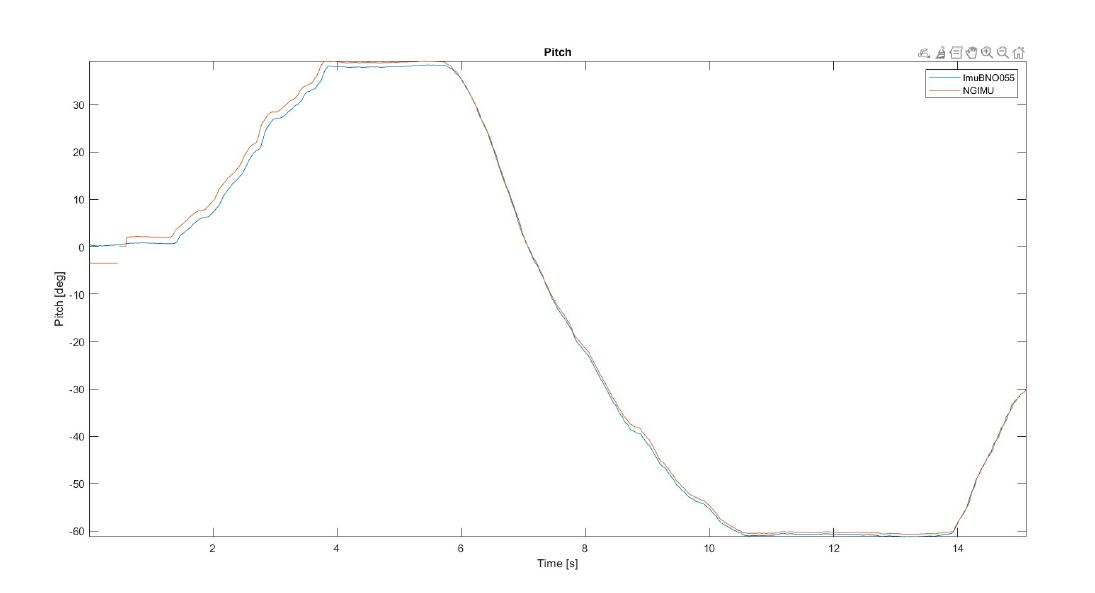
\includegraphics[width=0.8\textwidth,keepaspectratio]{figures/grafico.JPG}
\caption{Esempio di grafico}
\label{fig:grafico}
\end{figure}
\section{Test1}
Per ogni test riportate: cosa state testando, in che condizioni si è svolto il test, riferimenti a video/file di log che consegnate insieme a relazione e codice, grafici dei risultati, commento dei risultati.

\section{Test2}

\newpage
\addcontentsline{toc}{chapter}{Conclusioni e sviluppi futuri}
\section*{Conclusioni e sviluppi futuri}
Riassumere brevemente il lavoro svolto rispetto al task assegnato, evidenziando quali risultati sono stati raggiunti e quali no. Se ci sono aspetti del task non completati spiegare quali sono stati i problemi riscontrati in merito.\\
Inserire considerazioni personali su possibili sviluppi futuri dell'attività svolta (idee per migliorarla che non avete avuto modo di sperimentare, aspetti che suggerite di approfondire, problemi da risolvere..).

\addcontentsline{toc}{chapter}{Appendici}
\appendix
\chapter{Appendice1}
Se necessario ricorrete alle appendici per spiegare le parti "di contorno" dell'attività svolta e/o ciò che non riuscite ad inserire nello schema generale dei capitoli della relazione (es acquisizione dei dati con Matlab).


\bibliographystyle{ieeetr}
\bibliography{bibl} 
\end{document}
